\documentclass[12pt,a4paper]{book}
\usepackage[utf8]{inputenc}
%\usepackage[spanish, es-noquoting]{babel}
\usepackage[left=2.5cm,right=2.5cm,top=2.5cm,bottom=2.5cm]{geometry}
\usepackage{amsmath}
\usepackage{amsfonts}
\usepackage{amssymb}
\usepackage{amsthm, mathtools}
\usepackage{tikz,tikz-cd}
\usepackage{pdfpages}
\usepackage{adjustbox}
\usetikzlibrary{arrows, babel}
\usepackage{url}
\urlstyle{rm}
\usepackage[colorlinks=true,linktocpage=true,pagebackref=true,linkcolor=blue,urlcolor=blue]{hyperref}
\usepackage{graphicx}
%\usepackage{tocstyle}
%\usepackage{tocbibind}
%\usepackage{mathrsfs}
\usepackage[scr=boondox]{mathalfa}
\usepackage{anyfontsize}
\usepackage{epigraph}

%Fuente Palatino:
%\usepackage[sc]{mathpazo}
%Fuente Times:
\usepackage{newtxtext}
\usepackage{newtxmath}
%Fuente Libertine:
%\usepackage{libertine}
%\usepackage[libertine]{newtxmath}

\newtheorem{thm}{Theorem}[section]
\newtheorem{prop}[thm]{Proposition}
\newtheorem{lema}[thm]{Lemma}
\newtheorem{corol}[thm]{Corollary}
\theoremstyle{definition} \newtheorem{defn}[thm]{Definition}
\theoremstyle{definition} \newtheorem{ejemplo}[thm]{Example}
\theoremstyle{remark} \newtheorem{rem}[thm]{Remark}

\def\pr{\mathrm{pr}}
\def\OO{\mathscr{O}}
\def\AA{\mathscr{A}}
\def\BB{\mathscr{B}}
\def\LL{\mathscr{L}}
\def\VV{\mathscr{V}}
\def\MM{\mathscr{M}}
\def\II{\mathscr{I}}
\def\EE{\mathscr{E}}
\def\HH{\mathscr{H}}
\def\GG{\mathscr{G}}
\def\CC{\mathbf{C}}
\def\gg{\mathfrak{g}}
\def\ad{\mathrm{ad}}
\def\ZZ{\mathbf{Z}}
\def\RR{\mathbf{R}}
\def\KK{\mathbf{K}}
\def\SF{\mathbf{S}}
\def\TT{\mathbf{T}}
\def\NN{\mathbf{N}}
\def\PP{\mathbf{P}}
\def\tr{\mathrm{tr}}
\def\rk{\mathrm{rk}}
\def\id{\mathbf{1}}
\def\im{\mathrm{im}\ }
\def\Lie{\mathrm{Lie}}
\def\End{\mathrm{End}}
\def\Aut{\mathrm{Aut}}
\def\UU{\mathrm{U}}
\def\Nm{\mathrm{Nm}}
\def\SL{\mathrm{SL}}
\def\uu{\mathfrak{u}}
\def\Hom{\mathrm{Hom}}
\def\Bun{\mathbf{M}_{\mathrm{Bun}}}
\def\Hig{\mathbf{M}_{\mathrm{Higgs}}}
\def\MV{\mathbf{M}_{V}}
\def\SLHig{\mathbf{M}_{\mathrm{\SL(n,\CC)-Higgs}}}
\def\Sym{\mathrm{Sym}}
\def\Pic{\mathrm{Pic}}
\def\Spec{\mathrm{Spec}}
\def\RSpec{\mathbf{Spec}}
\def\Span{\mathrm{span}}
\def\Disc{\mathrm{Disc}}
\def\Res{\mathrm{Res}}
\def\delbar{\bar{\partial}}
\newcommand{\ve}[1]{\mathbf{#1}}

\let\emph\relax
\DeclareTextFontCommand{\emph}{\it\bfseries}

\DeclarePairedDelimiter\esc{\langle}{\rangle}
\DeclarePairedDelimiter\norm{\lVert}{\rVert}
\DeclarePairedDelimiter\abs{\lvert}{\rvert}

%%%        Otro formato para las secciones
\usepackage{titlesec}
\usepackage{remreset}

\renewcommand{\thechapter}{\Roman{chapter}}
\renewcommand{\thesection}{\arabic{section}}
\renewcommand{\thethm}{\thechapter.\thesection.\arabic{thm}}

\titleformat{\chapter}[block]
{\fontsize{20}{22}\bfseries\sffamily}
{\hfill CHAPTER \thechapter}
{1em}
{\vspace{1cm} \hrule\vspace{.5cm}\hfill}
[\vspace{.5cm}\hrule]


\titleformat{\section}[block]
{\fontsize{15}{18}\bfseries\sffamily\filcenter}
{\S\ \thesection.}
{1em}
{}

%\makeatletter
%\@removefromreset{section}{chapter}
%\makeatother
%%%

\title{Higgs bundles twisted by a vector bundle}
\author{Guillermo Gallego Sánchez}
\date{}


\begin{document}
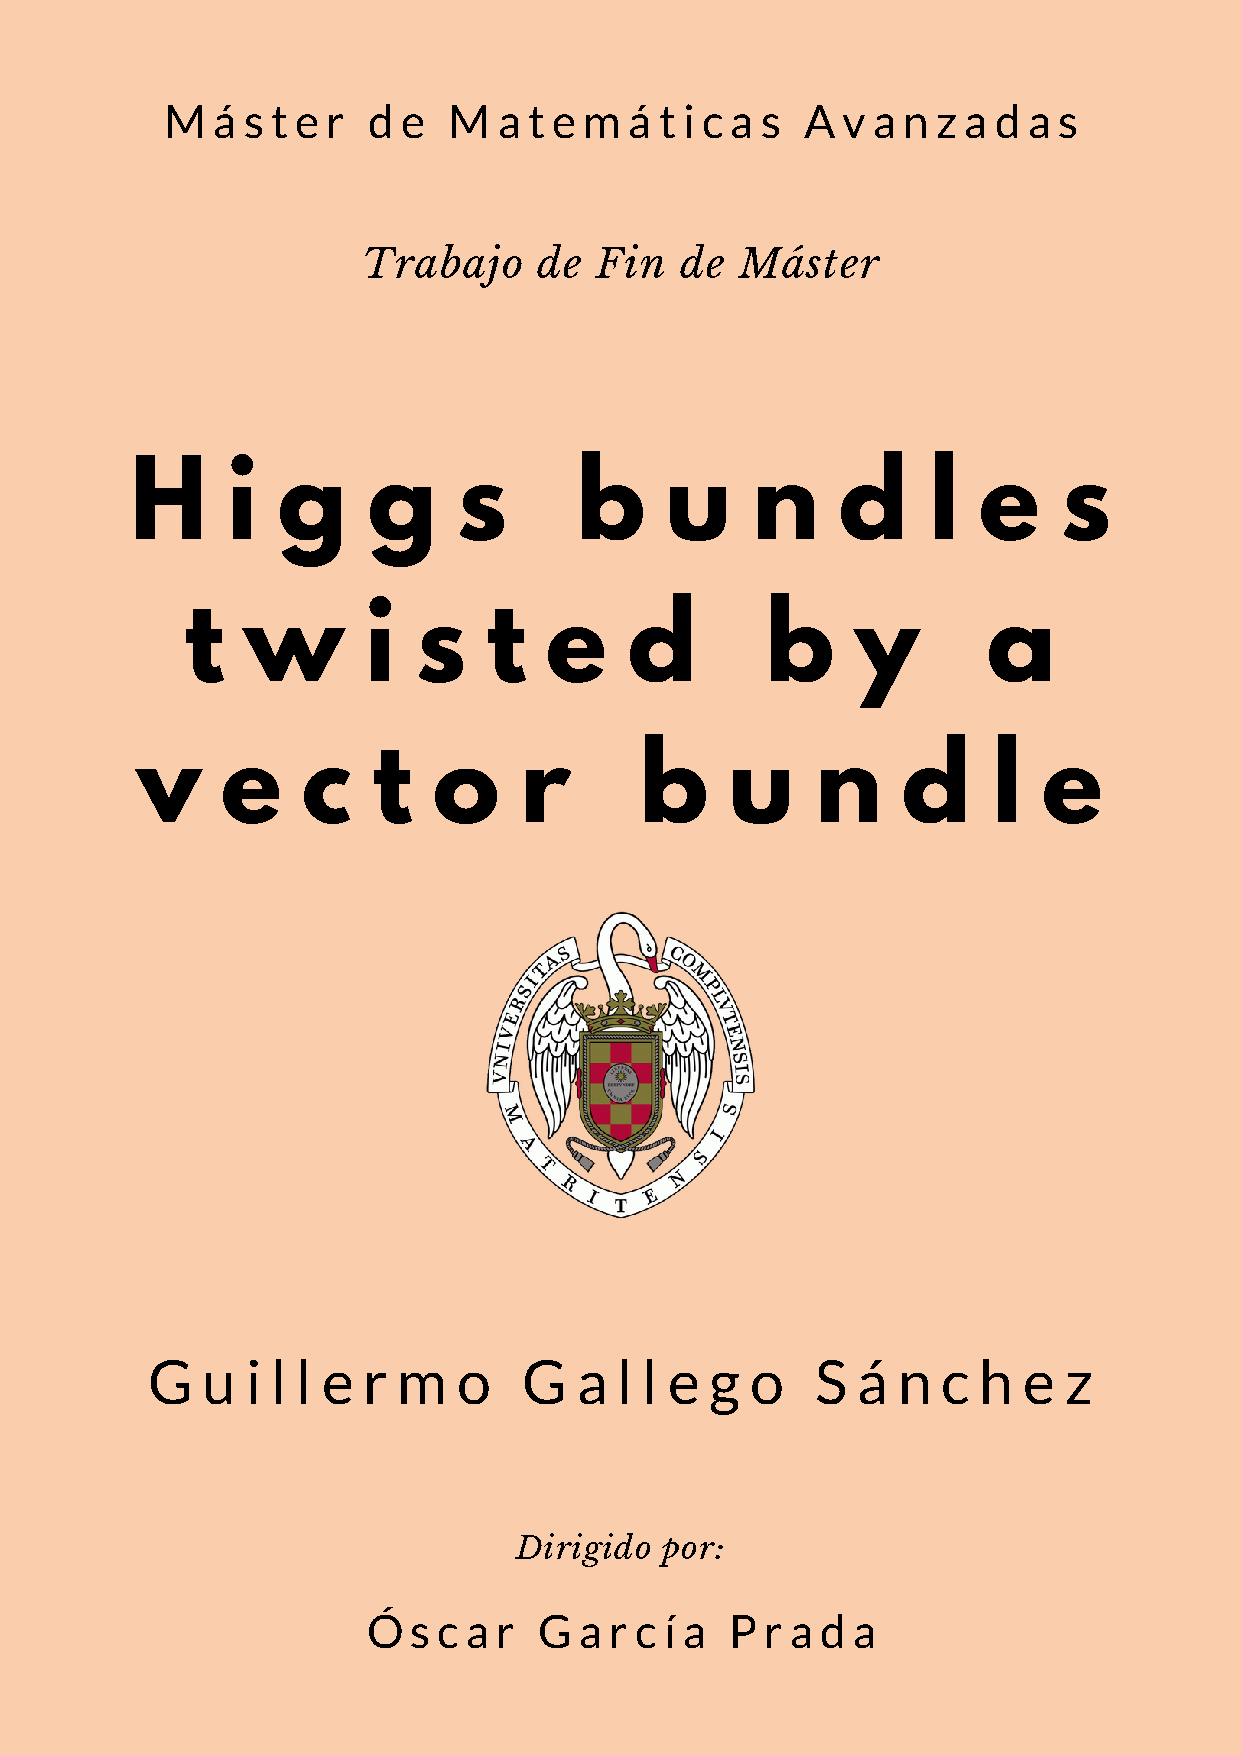
\includepdf[pages=-]{portada.pdf}
\begin{titlepage}
  \centering
%  \vspace*{1cm}
  \LARGE \textsc{Universidad Complutense de Madrid} \\
  \vspace{1cm}
  
\includegraphics[width=0.3\textwidth]{logoucm.png} \\
  \vspace{1cm}
  \LARGE \textit{Trabajo Final para optar al título de\\ \textbf{Máster de Matemáticas Avanzadas}} \\
  \vspace{1cm}

\rm \LARGE SEPTIEMBRE 2019

  \vspace{3cm}
  \hrule \vspace{0.5cm}
\Huge \bfseries \sffamily Higgs bundles twisted by a vector bundle \\
  \vspace{1cm}
\rm \Large \sffamily \it (Fibrados de Higgs torcidos por un fibrado vectorial) \\
   \vspace{0.5cm}\hrule

  \vfill

\begin{minipage}{0.5\textwidth}
  \rm \Large
  \textit{Autor:} \\
  Guillermo \textsc{Gallego Sánchez}
 \end{minipage}
 \hfill
\begin{minipage}{0.4\textwidth}
  \rm \large
  \textit{Director:}\\
Óscar \textsc{García Prada} \\
\textit{Tutor:} \\
Enrique \textsc{Arrondo Esteban}
  \end{minipage}
\end{titlepage}

\newpage\null\thispagestyle{empty}
\newpage\null\thispagestyle{empty}
\epigraph{\textit{¿Por ventura es asunto vano o es tiempo malgastado el que se gasta en vagar por el mundo, no buscando los regalos de él, sino las
asperezas por donde los buenos suben al asiento de la inmortalidad? [\dots] caballero soy y caballero he de morir si place al Altísimo. Unos van por el
ancho campo de la ambición soberbia; otros, por el de la adulación servil y baja; otros, por el de la hipocresía engañosa, y algunos, por el de la 
verdadera religión; pero yo, inclinado de mi estrella, voy por la angosta senda de la caballería andante, por cuyo ejercicio desprecio la hacienda, pero
no la honra. [\dots] yo soy enamorado [\dots] y, siéndolo, no soy de los enamorados viciosos, sino de los platónicos continentes. Mis intenciones siempre
las enderezo a buenos fines, que son de hacer bien a todos y mal a ninguno; si el que esto entiende, si el que esto obra, si el que desto trata merece
ser llamado bobo, díganlo vuestras grandezas.}}{Don Quijote de la Mancha}
\tableofcontents
\chapter{Vector bundles on Riemann surfaces}
\section{Topological classification of vector bundles}
The first step towards the classification of vector bundles on Riemann surfaces is their ``topological'' classification. That is, we want to classify smooth complex vector bundles on a Riemann surface up to $C^\infty$ isomorphism. This is in fact pretty easy to do, since the problem can be reduced to the classification of line bundles.
\begin{thm}
  If $E$ is a rank $n$ smooth complex vector bundle over a compact Riemann surface $X$ then it is isomorphic to $\det E \oplus (X\times \CC^{n-1})$.
\end{thm}
\begin{proof}
   We will proceed by induction on $n$. Of course, if $E$ is a line bundle, $E\cong \det E$. Now, take $n>1$, suppose that it is true for any vector bundle of rank $n-1$ and let $E$ be a rank $n$ vector bundle.
   \begin{lema}
     $E$ has a nowhere vanishing section.
   \end{lema}
   \begin{proof}
     Let $s_0$ be the zero section of $E$ and $S_0=s_0(X)\subset E$. By the transversality theorem \cite{hirsch}, we can densely choose a section $s\in \Gamma(E)$ transversal to $S_0$. Now, if $s$ vanishes at some point $x\in X$, then $s(x)\in S_0$ and, since $s$ is transversal to $S_0$, $$d_xs(T_xX) + T_{s(x)}S_0 = T_{s(x)}E.$$ But $\dim_\RR E=2n+2$, $\dim_\RR S_0 = 2$ and $\dim_\RR d_xs(T_xX) \leq \dim_\RR X = 2$, so, if $n>1$, dimensions do not add up to verify the above equality and therefore we get a contradiction. 
   \end{proof}

   Let us continue with the proof of the theorem. Since $E$ has a nowhere vanishing section $s$, we can define the line bundle
   \begin{equation*}
     L=\bigsqcup_{x\in X} \Span(s(x)),
   \end{equation*}
   with 
   \begin{align*}
      \pi:L&\longrightarrow X\\ 
       \lambda s(x) &\longmapsto x.
     \end{align*}
     Therefore, we can decompose $E=E'\oplus L$, with $E'$ a rank $n-1$ vector bundle. For example, fixing a metric on $E$, we can define $E'$ to be the orthogonal complement of $L$. But observe now that $L$ is isomorphic to the trivial line bundle: the bundle morphism
     \begin{align*}
      X\times \CC  &\longrightarrow L\\ 
	 (x,\lambda) &\longmapsto \lambda s(x), 
       \end{align*}
       is in fact an isomorphism. This can be proven by defining a metric on $L$ and normalizing $s \mapsto s/\norm{s}$. Then we can define the inverse
     $ y\in L \mapsto (\pi(y), \esc{s(\pi(y)),y})\in X\times \CC$. 

     Thus, we have shown that $E\cong E'\oplus (X\times \CC)$. Now, applying the induction hypothesis, $E'\cong \det E' \oplus (X\times \CC^{n-2})$, so $E\cong \det E' \oplus (X\times \CC^{n-1})$. Finally, via transition functions it can be easily shown that $\det E \cong \det E'$.
\end{proof}

This last theorem says that vector bundles can be topologically classified by their rank and their determinant, which is a line bundle. Let us proceed then with the classification of line bundles. Recall that all the data of a vector bundle can be recovered by the transition functions $\{g_{\alpha \beta}\in C^\infty(U_\alpha \cap U_\beta , \CC)\}$ defining it, where $\left\{ U_\alpha \right\}$ is an open cover of $X$. These functions verify the cocycle condition $$g_{\alpha \beta}=g_{\gamma \beta}\cdot g_{\alpha \gamma}.$$ Also recall that an isomorphism of vector bundles induces a coboundary on the transition functions
\begin{equation*}
  \tilde{g}_{\alpha\beta}=f^{-1}_{\delta\beta}\cdot g_{\gamma\delta} \cdot f_{\gamma\alpha}.
\end{equation*}
Therefore, topological ($C^\infty$) isomorphism classes of vector bundles are parametrized by the \v{C}ech cohomology group
\begin{equation*}
  H^1(X,C^{\infty,*}_X).
\end{equation*}
To obtain more information about this cohomology group we are going to introduce a very powerful tool: the first Chern class of a vector bundle.

Recall from Chern-Weil theory \cite{griffithsharris,wells} that for any complex vector bundle $E$ over $X$ and for any connection $\nabla$ on $E$ with associated curvature form $F$, the $2$-form $\tr F$ is closed and its de Rham cohomology class $[\tr F]\in H_{\mathrm{dR}}^2(X)$ does not depend on the choice of the connection, so it is an invariant of the vector bundle $E$. If we normalize this form to get an integer cohomology class, we can define the \emph{first Chern class} of $E$ as the cohomology class:
\begin{equation*}
  c_1(E)=\left[ \frac{i}{2\pi} \tr F \right] \in H_{\mathrm{dR}}^2(X).
\end{equation*}
We define the \emph{degree} of a vector bundle $E$ as the pairing of $c_1(E)$ with the fundamental class of $X$, that is
\begin{equation*}
  \deg E = \int_X\frac{i}{2\pi} \tr F. 
\end{equation*}
The next proposition \cite{wells} summarizes the most important properties about the degree that we are going to use:
\begin{prop}[Propierties of the degree]
  Let $E$ and $F$ be complex vector bundles over a compact Riemann surface $X$.
  \begin{enumerate}
    \item $\deg(E)$ depends only on the isomorphism class of $E$.
    \item $\deg(E) \in \mathbf{Z}$.
    \item $\deg(E\oplus F)=\deg(E)+ \deg(F)$.
    \item $\deg(E\otimes F)=\rk F \deg E + \rk E \deg F.$
    \item $\deg E=\deg(\det E) $.
    \item
      Let $\delta:H^1(X,C^{\infty,*}_X) \rightarrow H^2(X,\ZZ)$ be the connecting homomorphism of the long exact sequence in cohomology induced by the exponential sheaf exact sequence
      \begin{center}
	\begin{tikzcd}
	  0 \arrow{r} &	  \ZZ \arrow{r} & C^\infty_X \arrow{r}{\exp} & C^{\infty,*}_X \arrow{r} &0,
	 \end{tikzcd}
       \end{center}
       where $\exp(f)=e^{2\pi if}$.
      The diagram
      \begin{center}
	\begin{tikzcd}
	  H^1(X,C^{\infty,*}_X)	  \arrow{r}{\delta}\arrow{rd}[anchor=north,rotate=-30]{c_1} & H^2(X,\ZZ) \arrow[hook]{d}\\ 
	  & H^2_{\mathrm{dR}}(X),
	 \end{tikzcd}
       \end{center}
       is commutative.
  \end{enumerate}
\end{prop}

This last property will be crucial in the classification of line bundles. Let us consider again the exponential sheaf exact sequence
      \begin{center}
	\begin{tikzcd}
	  0 \arrow{r} &	  \ZZ \arrow{r} & C^\infty_X \arrow{r}{\exp} & C^{\infty,*}_X \arrow{r} & 0.
	 \end{tikzcd}
       \end{center}
       The existence of smooth partitions of unity implies that the sheaf $C^\infty_X$ is fine, so $H^1(X,C^\infty_X)=H^2(X,C^\infty_X)=0$. Therefore, the connecting map $\delta:H^1(X,C^{\infty,*}_X)\rightarrow H^2(X,\ZZ)$ is an isomorphism. If we now consider the set of integer de Rham cohomology classes, $H^2_{\mathrm{dR}}(X,\ZZ)$, which is just the image of $H^2(X,\ZZ)$ by the inclusion $H^2(X,\ZZ)\hookrightarrow H^2_{\mathrm{dR}}(X)$, we get an isomorphism $c_1:H^1(X,C_X^{\infty,*})\rightarrow H^2_{\mathrm{dR}}(X,\ZZ)$. Now, the isomorphism $H^2_{\mathrm{dR}}(X) \cong \CC$ given by integration on $X$, descends to an isomorphism $H^2_{\mathrm{dR}}(X,\ZZ) \cong \ZZ$.
    Summarizing, we have the diagram
       \begin{center}
	 \begin{tikzcd}
	   H^1(X,C_X^{\infty,*}) \arrow{r}{c_1} \arrow[bend right]{rr}{\deg}& H^2_{\mathrm{dR}}(X,\ZZ) \arrow{r}{\int_X} & \ZZ.
	 \end{tikzcd}
       \end{center}
       That is, the degree gives an isomorphism between the set isomorphism classes of smooth line bundles and $\ZZ$. This concludes the topological classification of vector bundles, which we can gather in the next theorem
       \begin{thm}
	 Smooth complex vector bundles over a compact Riemann surfaces are classified, up to $C^\infty$ isomorphism by their rank and their degree.
       \end{thm}
  
       \section{The problem of classification of holomorphic vector bundles}
       Now that we have classified vector bundles up to topological ($C^\infty$) isomorphism, we are going to pursue the full classification of holomorphic vector bundles over Riemann surfaces. According to the results of last section, we can reduce our problem to the study of the ``list'' of isomorphism classes of holomorphic vector bundles of fixed rank $n$ and degree $d$ (regarding them in particular as complex vector bundles). From the beginning, this problem gets really involved, since these ``lists'' are so big that they themselves admit a non-trivial geometric structure. These are the so called \emph{moduli spaces}. Therefore, the classification problem translates to that of investigating the geometric properties of the associated moduli spaces.

       To illustrate these ideas in more detail, let us consider the case of holomorphic line bundles. The same arguments regarding \v{C}ech cocycles of the previous section also apply now to show that the isomorphism classes of holomorphic vector bundles are parametrized by the sheaf cohomology group
       \begin{equation*}
	 H^1(X,\OO_X^*).
       \end{equation*}
       This cohomology group is called the \emph{Picard group} of $X$ and we denote it by $\Pic(X)$.
       Now, as before, we can consider the exponential sheaf sequence
      \begin{center}
	\begin{tikzcd}
	  0\arrow{r}&	  \ZZ \arrow{r} & \OO_X \arrow{r}{\exp} & \OO_X^* \arrow{r} & 0,
	 \end{tikzcd}
       \end{center}
       and the connecting operator $\delta:H^1(X,\OO_X^*)\rightarrow H^2(X,\ZZ)$ of the induced long exact sequence in cohomology. Analogously to the previous section, one can show that the diagram 
      \begin{center}
	\begin{tikzcd}
	  \Pic(X)	  \arrow{r}{\delta}\arrow{rd}[anchor=north,rotate=-30]{c_1} & H^2(X,\ZZ) \arrow[hook]{d}\\ 
	  & H^2_{\mathrm{dR}}(X)
	 \end{tikzcd}
       \end{center}
       is commutative. However, unlike the smooth case, the sheaf $\OO_X$ is not fine, since there are not holomorphic partitions of unity, so in general $\delta$ is not an isomorphism anymore. Let $\Pic^0(X)=\ker \delta \subset \Pic(X)$ be the subgroup of degree zero line bundles. Then, we have an exact sequence
      \begin{center}
	\begin{tikzcd}
	  0\arrow{r}&	  H^1(X,\ZZ) \arrow{r} & H^1(X,\OO_X) \arrow{r} & \Pic^0(X) \arrow{r}{\delta} & 0.
	 \end{tikzcd}
       \end{center}
       Therefore $\Pic^0(X)\cong H^1(X,\OO_X)/H^1(X,\ZZ)$. Now, the Dolbeaut theorem says that $H^1(X,\OO_X)\cong H^{0,1}(X)$ and the Hodge decomposition theorem says that $H^1(X,\CC)\cong H^{1,0}(X) \oplus H^{0,1}(X)$. Also, by Serre duality, $H^{1,0}(X)\cong H^{0,1}(X)^*$ and via Mayer-Vietoris one can easily prove that $H^1(X,\CC)\cong\CC^{2g}$ and that $H^1(X,\ZZ)\cong\ZZ^{2g}$, where $g$ is the genus of $X$. Putting all this together we have that $H^1(X,\OO_X)\cong \CC^{g}$, so $\Pic^0(X)$ is a complex torus. We call this complex torus 
       \begin{equation*}
	 J(X):=	 \frac{H^1(X,\OO_X)}{H^1(X,\ZZ)}
       \end{equation*}
       the \emph{Jacobian} of $X$. The other components of fixed degree of $\Pic(X)$ can be also shown to be isomorphic to the Jacobian of $X$, via the isomorphism
       \begin{align*}
	  \Pic^d(X)&\longrightarrow \Pic^0(X)\\ 
	   L &\longmapsto L\otimes M, 
	 \end{align*}
	 where $M \in \Pic^{-d}(X)$ is a fixed line bundle. It is of course injective, since if $L\otimes M \cong L'\otimes M$, then 
	 \begin{equation*}
	   L\cong L\otimes M \otimes M^* \cong L' \otimes M \otimes M^* \cong L',
	 \end{equation*}
	 and it is also surjective since for every line bundle $L \in \Pic^0(X)$, $L\cong (L\otimes M^*) \otimes M$.
       
	 The result for line bundles already hints on the complexity of the general problem. However, for very low genus the problem can be solved relatively easily. For genus 0, Grothendieck proved that every holomorphic vector bundle on the Riemann sphere $\PP^1_\CC$ can be decomposed as a direct sum of line bundles. A proof of this result can be found in \cite{hartshorne}. For genus 1, it was Atiyah \cite{atiyahelliptic} who showed that the ``moduli space'' of indecomposable vector bundles with fixed rank and degree over an elliptic curve is isomorphic to the curve itself. 

	 The problem gets its full complexity in the case of general genus $g\geq 2$, for which we will dedicate the rest of the chapter. To construct a ``good'' moduli space (one with nice topological properties, like being Hausdorff) we need to consider the idea of stability, arising from Mumford's Geometric Invariant Theory \cite{git}. This theory also allows to construct the moduli space of stable vector bundles, although it can also be done using analytic methods \cite{kobayashi}. This moduli space has very nice and interesting geometric properties and it has been studied from the algebraic point of view (for example in the works of Narasimhan, Ramanan or Seshadri) as well as from the analytical or gauge-theoretical point of view (by Atiyah, Bott, Donaldson or Hitchin, for example).

	 \section{Holomorphic structures as Dolbeaut operators}
	 Let $\ve{E}$ be a holomorphic vector bundle on a compact Riemann surface $X$. Associated to $\ve{E}$, we have the \emph{Dolbeaut operator}
	 \begin{align*}
	   \delbar_\ve{E}:\Omega^{p,q}(X,\ve{E})&\longrightarrow \Omega^{p,q+1}(X,\ve{E})
	   \end{align*}
	   which satisfies
	   \begin{equation*}
	     \delbar_{\ve{E}}(\alpha\psi)=(\delbar \alpha)\psi + (-1)^{p} \alpha \wedge \delbar_{\ve{E}} \psi,
	   \end{equation*}
	   for every $\alpha \in \Omega^p(X)$, $\psi \in \Gamma(\ve{E})$, and 
	   \begin{equation*}
	     \delbar_{\ve{E}}^2=0.
	   \end{equation*}

	   Conversely, if $E$ is a complex vector bundle, any operator $\delbar_{\ve{E}}:\Omega^{p,q}(X,E)\rightarrow \Omega^{p,q+1}(X,E)$ which satisfies the conditions above induces on $E$ the structure of a holomorphic vector bundle. The idea here is that $\delbar_{\ve{E}}^2=0$ is the \emph{integrability condition} for the PDE $\delbar_{\ve{E}} s=0$ (check out \cite{donaldson4manifolds}  for a proof of this fact). The solutions of this PDE are the holomorphic vector functions, so the sheaf of local solutions is locally free over $\OO_X$ and therefore it is an holomorphic vector bundle supported on $E$. In conclusion, if we define $\AA_{\delbar}$ as the set of all such $\delbar_{\ve{E}}$ operators satisfying the previous conditions, this set is in bijection with the set of all holomorphic structures on $E$.

	   Now let us consider the group $\GG^c$ of \emph{gauge transformations} of a complex vector bundle $E$, that is, diffeomorphisms $g:E\rightarrow E$ such that the diagram
	   \begin{center}
	     \begin{tikzcd}
	       E \arrow{rr}{g} \arrow{rd} && E \arrow{ld}	       \\ 
	       & X &
	     \end{tikzcd}
	   \end{center}
	   commutes. That is, $\GG^c=\Gamma(\Aut(E))$. This group acts on $\AA_{\delbar}$ by the rule
	   \begin{equation*}
	     g\cdot \delbar_{\ve{E}}=g\delbar_{\ve{E}} g^{-1}.
	   \end{equation*}
	   Therefore we can identify the quotient set $\AA_{\delbar}/\GG^c$ with the set of isomorphism classes of holomorphic vector bundles of rank $\rk E$ and degree $\deg E$. Even though $\AA_{\delbar}$ and $\GG^c$ are infinite-dimensional spaces, using analytic techniques \cite{kobayashi} they can be given the structure of \emph{Banach manifolds} (roughly, spaces locally modeled by Banach spaces) and this quotient space can be precisely constructed. This has however a serious problem: the obtained space is not Hausdorff. Nevertheless, if we restrict ourselves to the class of \textit{stable} vector bundles, with the same analytic methods we can obtain a ``good'' moduli space.
	   \begin{defn}[Stable vector bundles]
	     Let $E$ be a complex vector bundle over a compact Riemann surface $X$. We define the \emph{slope} of $E$ as the number
	     \begin{equation*}
	       \mu(E)=\deg E/ \rk E.
	     \end{equation*}
	     We say that a holomorphic vector bundle $\ve{E}=(E,\delbar_{\ve{E}})$ is \emph{stable} if for every proper holomorphic subbundle $\ve{E}'\subset \ve{E}$ (that is, for every subbundle $E'\subset E$ such that $\delbar$ preserves $E'$), $$\mu(E')<\mu(E).$$ 
	     Let $n=\rk E$ and $d=\deg E$. We consider $\AA_{\delbar}^s\subset \AA_{\delbar}$ the subset of stable holomorphic bundles $\ve{E}=(E,\delbar_{\ve{E}})$ and define the \emph{moduli space of stable holomorphic vector bundles} of rank $n$ and degree $d$ as the quotient
	     \begin{equation*}
	       \Bun(n,d)=\AA_{\delbar}^s/\GG^c.
	     \end{equation*}
	   \end{defn}
	   
	   Using analytic methods \cite{kobayashi} one can show
	   \begin{thm}\label{modulibundles}
	     The moduli space $\Bun(n,d)$ is a complex manifold of dimension $1+n^2(g-1)$, where $g$ is the genus of $X$.
	   \end{thm}

	   \section{Deformations of holomorphic structures}\label{deformationsholomorphic}
	   In this section we are going to compute the dimension of $\Bun(n,d)$, stated in Theorem \ref{modulibundles}, using deformation theory. The idea is to identify the tangent space of $\Bun(n,d)$ at some point $\delbar_\ve{E}$ and find its dimension. 

	   In first place, observe that $\AA_{\delbar}$ is an affine space modelled on $\Omega^{0,1}(X,\End\ E)$. Therefore, the tangent space of $\AA_{\delbar}$ at $\delbar_{\ve{E}}$ is isomorphic to $\Omega^{0,1}(X,\End\ E)$. Now, let $\Lie\ \GG^c = \Gamma(\End\ E)$ be the Lie algebra of $\GG^c$ and pick an element $\xi \in \Gamma(\End\ E)$. Let us compute the action of this element on the tangent space $\Omega^{0,1}(X,\End\ E)$,
	   \begin{equation*}
	     \left. \frac{d}{dt} \right|_{t=0} \exp(\xi t)  \delbar_{\ve{E}} \exp(-\xi t) = -\delbar_\ve{E} \xi.
	   \end{equation*}
	   Hence, since stability is an open condition, the tangent space $T_{\delbar_{\ve{E}}}\Bun(n,d)$ is isomorphic to
	   \begin{equation*}
	     H^1(X,\End\ \ve{E})=\frac{\Omega^{0,1}(X,\End\ E)}{\delbar_\ve{E} \Gamma(\End\ E)}.
	   \end{equation*}

	   To compute the dimension of this tangent space, we use the \emph{Riemann-Roch theorem}
	   \begin{equation*}
	     \dim H^0(X,\End\ \ve{E}) - \dim H^1(X,\End\ \ve{E})=\deg(\End\ \ve{E}) + \rk(\End\ \ve{E})(1-g).
	   \end{equation*}
	   Now, note that $\End\ E=\Hom(E,E)\cong E^*\otimes E$, so
	   \begin{equation*}
	     \rk(\End\ E)=n^2
	   \end{equation*}
	   and
	   \begin{equation*}
	     \deg(\End\ E)=\rk(E^*)\deg(E) + \rk(E)\deg(E^*)=n\deg E - n\deg E=0.
	   \end{equation*}
	   Therefore
	   \begin{equation*}
	     \dim H^0(X,\End\ \ve{E}) - \dim H^1(X,\End\ \ve{E})=n^2(1-g).
	   \end{equation*}

	   To find the dimension of $H^0(X,\End\ \ve{E})$ we use the following result:
	   \begin{prop}
	     If $\ve{E}$ is a stable holomorphic vector bundle, then
	     \begin{equation*}
	       H^0(X,\End\ \ve{E})=\CC.
	     \end{equation*}
	   \end{prop}
	   \begin{proof}
	     What we will see is that every endomorphism is a scalar multiple of the identity $\id_{\ve{E}}$. Pick any endomorphism $f:\ve{E}\rightarrow \ve{E}$ and let $\lambda \in \CC$ be an eigenvalue of $f_x:\ve{E}_x \rightarrow \ve{E}_x$. Let us define the endomorphism $g=f-\lambda \id_{\ve{E}}$. Since $\lambda$ is an eigenvalue of $f_x$, we have $\det g_x=0$. 
	     Assuming that $g$ is nonzero, we will prove that $g$ is injective and hence $\det g_x\neq 0$ arriving at a contradiction.
	     To see this, suppose that $\im g \subset \ve{E}$ is a holomorphic strict subbundle of $\ve{E}$. Then, since $\ve{E}$ is stable, $\mu(\im g) < \mu(\ve{E})$. But we also have that $\mu(\ve{E})<\mu(\im g)$, so $\mu(\ve{E})<\mu(\ve{E})$ and we have a contradiction. Therefore $g$ is injective.	     
	     We conclude then that $g=0$, so $f=\lambda\id_{\ve{E}}$.
	   \end{proof}

	   Finally, we get
	   \begin{equation*}
	     \dim \Bun(n,d)=\dim H^1(X,\End\ \ve{E})= 1+n^2(g-1).
	   \end{equation*}


	   

	   \section{Holomorphic structures and unitary connections}
	   Although we will not enter into detail, the main reason why the quotient $\AA_{\delbar}/\GG^c$ is not Hausdorff and why we need to introduce the stability condition is that the group $\GG^c=\Gamma(\Aut(E))$ is a complex group. Indeed, it is the complexification of the group $\GG=\Gamma(\UU_h(E))$, where $h$ is a Hermitian metric on $E$ and $\UU_h(E)$ is the subgroup of $\Aut(E)$ consisting on automorphisms of $E$ preserving the metric $h$. The idea for this is essentially that the general linear group $\mathrm{GL}(n,\CC)$ is the complexification of the unitary group $\mathrm{U}(n)$. This motivates the study of unitary connections,
which will give a gauge-theoretical approach to holomorphic vector bundles. This will allow us to give another analytical construction of the moduli space, this time as the space of solutions (up to gauge equivalence) to some differential equation.

Let $\ve{E}=(E,\delbar_{\ve{E}})$ be a holomorphic vector bundle on $X$ and let $h$ be a Hermitian metric on $E$. Recall that for any connection $\nabla:\Gamma(E) \rightarrow \Omega^1(X,E)=\Omega^{1,0}(X,E) \oplus \Omega^{0,1}(X,E)$ on $E$ there is a natural splitting $\nabla=\nabla^{1,0}+\nabla^{0,1}$, where
\begin{align*}
  \nabla^{1,0}:\Gamma(E) \longrightarrow \Omega^{1,0}(X,E), \\
  \nabla^{0,1}:\Gamma(E) \longrightarrow \Omega^{0,1}(X,E).
\end{align*}
The \emph{Chern connection} in $(\ve{E},h)$ is the unique $h$-\emph{unitary} connection (that is, $$d\esc{\xi,\eta}=\esc{\nabla \xi,\eta} + \esc{\xi,\nabla \eta},$$ for $\xi, \eta$ local sections of $E$) such that $$\nabla^{0,1}= \delbar_{\ve{E}}:\Gamma(E) \rightarrow \Omega^{0,1}(X,E).$$ Go to \cite{wells} for a proof of the existence and uniqueness of this connection. 

Conversely, given any $h$-unitary connection $\nabla$ on $E$, we can define a holomorphic structure by fixing $\delbar_{\ve{E}}=\nabla^{0,1}$ and extending to operators $\Omega^{p,q}(X,E) \rightarrow \Omega^{p,q+1}(X,E)$ by linearity. Therefore, the set holomorphic structures on $E$ can be identified with the set $\AA_h$ of all $h$-unitary connections on $E$.

Note now that the curvature of any connection on $E$ must satisfy that the cohomology class
\begin{equation*}
  [\tr F] = -i2\pi c_1(E).
\end{equation*}
Fixing an area form $\omega_X$ on $X$ so that $\int_X \omega_X=1$, we can choose a representative of $c_1(E)$ of the form $k\omega_X$, where $k\in \CC$ is a constant. Of course,
\begin{equation*}
  \deg E = \int_X c_1(E) = \int_X k\omega_X=k,
\end{equation*}
so $k=\deg E$. Therefore we can ask if there is a connection on $E$ such that its curvature satisfies
\begin{equation*}
  \tr F = -2\pi i\deg(E) \omega_X.
\end{equation*}
Or, more generally, if $\id_{E}$ denotes the identity endomorphism of $E$, we can ask whether 
\begin{equation*}
  F = -2\pi i\frac{\deg E}{\rk E} \id_E \omega_X.
\end{equation*}
Recall that we defined the number $\mu(E)=\deg E /\rk E$ as the slope of $E$. 

\begin{defn}
  We say that a connection $\nabla$ on a complex vector bundle $E$ has \emph{constant central curvature} if is curvature $F$ satisfies
  \begin{equation*}
    F=-2\pi i \mu(E) \id_E \omega_X.
  \end{equation*}
  In particular, if $\deg E=0$, $F=0$ and we say that $\nabla$ is a \emph{flat connection}.
\end{defn}

Finally, we want to consider connections that are \textit{irreducible}:
\begin{defn}
  A unitary connection $\nabla$ on a complex Hermitian vector bundle $(E,h)$ is \emph{reducible} if $(E,h)=(E_1,h_1)\oplus (E_2,h_2)$ and $\nabla=\nabla_1\oplus \nabla_2$. We say that $\nabla$ is \emph{irreducible} if it is not reducible.
\end{defn}

Let us consider then the set $\AA_h^s$ of all $h$-unitary irreducible connections of central constant curvature on $E$. The gauge group $\GG$ acts on connections by conjugation $\nabla \mapsto g\nabla g^{-1}$, $g\in \GG$, and this action preserves irreducibility and the equation of constant central curvature, so the group $\GG$ acts on $\AA_h^s$. Now, the same analytic techniques mentioned in the previous section \cite{kobayashi} allow us to construct a ``good'' quotient:
\begin{thm}
  The moduli space of irreducible constant central curvature unitary connections $\AA_h^s/\GG$ on $(E,h)$ has the structure of a smooth real manifold of dimension $2+2n^2(g-1)$, where $n=\rk E$ and $g$ is the genus of $X$.
\end{thm}

Now, Donaldson's version of the theorem of Narasimhan-Seshadri relates this moduli space with the moduli space of stable holomorphic vector bundles.

\begin{thm}[Donaldson-Narasimhan-Seshadri]\label{narasimhanseshadri}
  Let $(E,h)$ be a Hermitian complex vector bundle of rank $n$ and degree $d$ on a compact Riemann surface $X$. An irreducible unitary connection $\nabla$ has constant central curvature if and only if the associated holomorphic vector bundle $(E,\nabla^{0,1})$ is stable.
\end{thm}
This can be reformulated in terms of moduli spaces:
\begin{corol}
  The map
  \begin{align*}
    \AA_h&\longrightarrow \AA_{\delbar}\\ 
     \nabla &\longmapsto \nabla^{0,1}, 
    \end{align*}
    descends to a homeomorphism
    \begin{equation*}
      \AA_h^s/\GG \cong \AA^s_{\delbar} /\GG^c = \Bun(n,d).
    \end{equation*}
\end{corol}
We will prove the ``easy'' direction of the equivalence. The proof in the other direction consists in defining a Yang-Mills functional and looking for a minimum of it using analytic techniques, in particular a theorem by Uhlenbeck \cite{uhlenbeck}. Check \cite{donaldson} for the details.
\begin{proof}
First, let us suppose that $\nabla$ has constant central curvature
\begin{equation*}
  F=-2\pi i \frac{d}{n} \id_E \omega_X,
\end{equation*}
and define $\delbar_{\ve{E}}=\nabla^{0,1}$. Let $E'\subset E$ be a subbundle preserved by $\delbar_{\ve{E}}$. The Hermitian metric gives a smooth splitting
\begin{equation*}
  E=E'\oplus E'',
\end{equation*}
and we can write
\begin{equation*}
  \delbar_{\ve{E}}=\left(
  \begin{array}{cc}
    \delbar_{\ve{E}'} & \beta \\
    0 & \delbar_{\ve{E}''}
  \end{array}\right),
\end{equation*}
where $\delbar_{\ve{E}'}$ and $\delbar_{\ve{E}''}$ are the restrictions of $\delbar_{\ve{E}}$ to $E'$ and $E''$ and $\beta \in \Omega^{0,1}(X,\Hom (E'',E'))$. Now $\nabla$ can be written as
\begin{equation*}
  \nabla=\left(
  \begin{array}{cc}
    \nabla_{E'} & \beta \\
    -\beta^\dagger & \nabla_{E''}
  \end{array}\right),
\end{equation*}
where $\nabla_{E'}$ and $\nabla_{E''}$ are the connections associated to $\delbar_{\ve{E}'}$ and $\delbar_{\ve{E}''}$ and $$\beta^\dagger=\star \bar{\beta} \in \Omega^{1,0}(X,\Hom(E',E''))$$ is the transpose (on the matrix part) conjugate (on the form part) of $\beta$. The curvature of $\nabla$ can be written now as
\begin{equation*}
  F=\left(
  \begin{array}{cc}
    F_{E'}-\beta \beta^\dagger & \nabla_{\Hom(E'',E')}\beta \\
    -\nabla_{\Hom (E',E'')}\beta^\dagger & F_{E''}-\beta^\dagger  \beta
  \end{array}\right)=-2\pi i\frac{d}{n} \id_E \omega_X,
\end{equation*}
where we understand $\beta \beta^\dagger$ as $BB^\dagger \otimes \alpha \wedge \bar{\alpha}$, where $B \in \Hom(E'',E)$ and $\alpha \in \Omega^{0,1}(X)$ (take a look at Remark \ref{obsproducto}).
The first corner of this equality now says that
\begin{equation*}
  F_{E'}-\beta\beta^\dagger = -2\pi i \frac{d}{n} \id_{E'} \omega_X.
\end{equation*}
Taking the trace and integrating we get
\begin{equation*}
  \frac{i}{2\pi}\int_X \tr F_{E'} - \frac{i}{2\pi} \int_X \tr(\beta \beta^\dagger) = d\frac{\rk E'}{n}.
\end{equation*}
Therefore
\begin{equation*}
  \frac{\deg E'}{ \rk E'} = \frac{d}{n} + \frac{i}{2\pi} \int_X \tr(\beta \beta^\dagger).
\end{equation*}
Now, $\tr(\beta\beta^\dagger)$ is precisely $- \norm{\beta}^2 \omega_X$. Thus we have proven that 
\begin{equation*}
\mu(E')= \mu(E) - \norm{\beta}^2 .
\end{equation*}
The connection $\nabla$ is irreducible, so $\norm{\beta}\neq 0$ and $\mu(E')< \mu(E)$. That is, $E$ is stable.
\end{proof}

\chapter{Momentum maps and symplectic quotients}
\section{Banach manifolds}
For the purpose of this text it is necessary to work on an infinite-dimensional context, so we can construct the moduli spaces as quotients of infinite-dimensional manifolds. To do this, we need to consider an infinite-dimensional analogous to differential calculus and the notion of an infinite-dimensional smooth manifold. Here we just state the basic definitions and results, which are a direct generalization of the classical ones, and refer to \cite{abrahammarsdenratiu,lang} for more details.
\begin{defn}
  Let $E$ and $F$ be Banach spaces and $U\subset E$ an open set. Let $f:E\rightarrow F$ be a continuous map. We say that $f$ is \emph{differentiable} at a point $x_0 \in U$ if there exists a continuous linear map $d_{x_0}f:E\rightarrow F$ such that 
  \begin{equation*}
    \lim_{h\rightarrow 0} \frac{\norm{f(x_0+h)-f(x_0)-d_{x_0}f(h)}_F}{\norm{h}_E}=0.
  \end{equation*}
  If this map $d_{x_0}f$ exists, then it is unique and it is called the \emph{derivative of $f$ at $x_0$}.
  If $f$ is differentiable at every point of $U$, then we have a map
  \begin{align*}
    df :U&\longrightarrow L(E,F)\\ 
      x &\longmapsto d_xf, 
    \end{align*}
    where $L(E,F)$ denotes the set of bounded linear maps $E\rightarrow F$. If $df$ is continuous, we say that $f$ is \emph{of class} $C^1$. Inductively, we define maps of class $C^p$, for $p\in \mathbf{N} \cup \left\{ \infty \right\}$. If $f$ is of class $C^{\infty}$, we say that it is \emph{smooth}. If $f$ is a bijective map of class $C^p$ such that its inverse is also of class $C^p$, we say that $f$ is a $C^p$-\emph{diffeomorphism}. If we do not specify, by a \emph{diffeomorphism} we just mean a $C^\infty$-diffeomorphism.
\end{defn}

As we said before, all the basic definitions and results of classical differential calculus (the chain rule, Taylor's formula, inverse and implicit function theorems etc.) can be generalized to the infinite-dimensional context. 
%\begin{thm}[Inverse function theorem]
%  Let $X$, $Y$ be Banach spaces, $U\subset X$ open and $f:U\rightarrow Y$ a map of class $C^p$, for some $p\in \mathbf{N}\cup \{\infty\}$. Assume that for some point $x_0 \in U$ the derivative $d_{x_0}f:X\rightarrow Y$ is a bounded linear isomorphism. Then $f$ is a local $C^p$-diffeomorphism at $x_0$.
%\end{thm}

\begin{defn}
  Let $X$ be a Hausdorff topological space. An \emph{atlas of class} $C^p$ on $X$ is a collection of \emph{charts} $(U_\alpha,\varphi_\alpha)$ such that
  \begin{enumerate}
    \item The $U_\alpha\subset X$ are open subsets of $X$, and $X=\bigcup_\alpha U_\alpha$.
    \item Each $\varphi_\alpha:U_\alpha \rightarrow V_\alpha$ is a homeomorphism of $U_\alpha$ onto some open subset of a Banach space $V_\alpha \subset E_\alpha$ and for any $\alpha, \beta$, $\varphi_\alpha(U_\alpha \cap U_\beta)$ is open in $E_\alpha$.
    \item The map 
      \begin{equation*}
	\varphi_\beta \circ \varphi_\alpha ^{-1}:\varphi_\alpha(U_\alpha \cap U_\beta) \rightarrow \varphi_\beta(U_\alpha \cap U_\beta)
      \end{equation*}
      is a $C^p$-diffeomorphism for each pair of indices $\alpha,\beta$.
  \end{enumerate}
\end{defn}
Compatibility classes for this kind of atlases are defined like in the finite-dimensional case. An equivalence class of this atlases (or a maximal atlas) is what gives $X$ the structure of a $C^p$-\emph{Banach manifold}. A $C^\infty$-Banach manifold is what we call a \emph{Banach smooth manifold}.

Let $X$ be a Banach smooth manifold and $x\in X$. Consider triples $(U,\varphi,v)$, where $(U,\varphi)$ is a chart at $x$ with $\varphi:U\rightarrow E$, $E$ a Banach space, and $v\in E$. We say that two such triples $(U,\varphi,v)$ and $(U',\varphi',v')$ are \emph{equivalent} if 
\begin{equation*}
  d_{\varphi(x)}(\varphi'\circ \varphi^{-1})(v)=v'.
\end{equation*}
The chain rule guarantees that this is an equivalence relation and an equivalence class is called a \emph{tangent vector of $X$ at $x$}. The set of these equivalence classes is denoted by $T_xX$  and it acquires the structure of a Banach space via the bijection $[(U,\varphi,v)]\leftrightarrow v$. We call this space the \emph{tangent space of $X$ at $x$}.

\begin{rem}
  As one can notice, the previous definition is analogous to one of the classical definitions of the tangent space. However, not all the classical definitions coincide in the infinite-dimensional setting. For example, although in general this definition can be seen to coincide with the one given as equivalence classes of curves with the same velocity, it does not coincide with the one given using derivations. In a general case in which the model space is not reflexive there are more derivations than tangent vectors.
\end{rem}

Now that we have a good notion of what the tangent space is in an infinite-dimensional setting one can give all the typical constructions derivated from it just like in the classical theory. In that way we can generalize to the context of Banach manifolds the notions of the tangent and cotangent bundles and all its tensor powers, vector fields, differential forms, the $d$ operator, the induced maps on these sets, etc. 

To finish the section, we generalize the notion of a Lie group. A \emph{Banach Lie group} is a Banach smooth manifold that has a group structure consistent with its manifold structure, that is, such that the group multiplication
\begin{align*}
   G\times G&\longrightarrow G\\ 
    (g,h) &\longmapsto gh 
  \end{align*}
  is a smooth map.
  As in the classical case, the \emph{Lie algebra} $\gg$ of $G$ is just the tangent space at the identity $T_eG$, which again happens to be isomorphic to the space the set of (left) invariant vector fields, so it is naturally equipped with a \emph{Lie bracket}.

  \section{Symplectic manifolds and the momentum map}
  \begin{defn}
    Let $X$ be a Banach smooth manifold. A \emph{symplectic form} on $X$ is a non-degenerate closed $2$-form on $X$, that is, a $2$-form $\omega$ satisfying:
    \begin{enumerate}
      \item For each $x\in X$, $\omega_x:T_xX \times T_xX \rightarrow \RR$ is continuous;
      \item For each $x\in X$, $\omega_x$ is non-degenerate, i.e., if $\omega_x(u,v)=0$ for all $v\in T_xX$, then $u=0$;
      \item $\omega_x$ is smooth in $x$;
      \item $\omega$ is closed, i.e., $d\omega=0$.
    \end{enumerate}
    The pair $(X,\omega)$ is called a \emph{symplectic manifold}.
  \end{defn}

  Note that the form $\omega_x$ defines a bounded linear map 
  \begin{align*}
     T_xX&\longrightarrow T_xX^*\\ 
      v &\longmapsto \omega(v,-). 
    \end{align*}
Unlike in the finite-dimensional case, the non-degeneracy condition does not imply that this map is bijective, although it does imply that it is injective.

\begin{ejemplo}\label{cotangente}
The cotangent space $T^*M$ of any smooth manifold can be endowed with a symplectic structure in the following way. We first consider the bundle projection $\pi:T^*M\rightarrow M$ and the pull-back bundle
\begin{center}
  \begin{tikzcd}
\pi^*T^*M    \arrow{rr}\arrow{dd} && T^*M \arrow{dd} \\ 
     && \\
     T^*M \arrow{rr}[anchor=south]{\pi} && M.
   \end{tikzcd}
 \end{center}
 This bundle has a tautological section $\theta\in \Gamma(T^*M,\pi^*T^*M)$: $\theta(y)=(y,y)$ for each $y \in T^*M$. The differential of this section $\omega=d\theta$ is a symplectic form on $T^*M$. Locally, if $M$ is finite-dimensional and $(x_1,\dots,x_n)$ are coordinates on $M$ and cotangent vectors are parametrized by coordinates $(y_1,\dots,y_n)$, the form $\theta$ is defined by
 \begin{equation*}
   \theta=\sum_{i=1}^n y_i dx_i,
 \end{equation*}
 and
 \begin{equation*}
   \omega=\sum_{i=1}^n dy_i \wedge dx_i.
 \end{equation*}
 \qed
\end{ejemplo}

We say that a vector field $\ve{v}:X\rightarrow TX$ on a symplectic manifold $(X,\omega)$ is \emph{symplectic} if the Lie derivative $L_{\ve{v}} \omega$ vanishes, that is, if
\begin{equation*}
  L_{\ve{v}} \omega = d(i_{\ve{v}} \omega) + i_{\ve{v}} (d\omega)=0,
\end{equation*}
where $i_{\ve{v}}$ denotes the contraction. Since $\omega$ is closed, $\ve{v}$ is symplectic if and only if the $1$-form $i_{\ve{v}} \omega$ is closed. We say that $\ve{v}$ is \emph{Hamiltonian} if $i_{\ve{v}} \omega$ is exact. In that case, there exists a function $f:X\rightarrow \RR$, called the \emph{Hamiltonian} of $\ve{v}$ such that
\begin{equation*}
  df=-i_{\ve{v}} \omega.
\end{equation*}
The minus sign in the last equality is just a widely used convention. Of course, if the first de Rham cohomology of $X$ vanishes, $H^1_{\mathrm{dR}}(X)=0$, then every symplectic vector field is Hamiltonian. In particular, every symplectic vector field is \emph{locally Hamiltonian}. Reciprocally, to every function $f:X\rightarrow \RR$, we can define the \emph{Hamiltonian vector field associated to $f$} as the vector field $\ve{v}_f$ determined by the equation
\begin{equation*}
  df=-i_{\ve{v}_f}\omega.
\end{equation*}
Given two functions $f$ and $g$, we define their \emph{Poisson bracket} as the function
\begin{equation*}
  \left\{ f,g \right\}=\ve{v}_f g = -\ve{v}_g f = -\left\{ g,f \right\}.
\end{equation*}
Two functions are said to \emph{Poisson commute} if $\{f,g\}=0$.

\begin{ejemplo}
  We can consider the cotangent bundle $T^*M$ of some manifold $M$ with the canonical symplectic structure $\omega=\sum dy_i \wedge dx_i$. If $f$ and $g$ are functions of $(y_1,\dots,y_n)$ alone,
  \begin{equation*}
    df=\sum_i \frac{\partial f}{\partial y_i} dy_i =- i_{\ve{v}_f}\omega
  \end{equation*}
  so
  \begin{equation*}
    \ve{v}_f=\sum_i \frac{\partial f}{\partial y_i}\frac{\partial}{\partial x_i}.
  \end{equation*}
  Thus, 
  \begin{equation*}
    \left\{ f,g \right\}=\ve{v}_f g=\sum_{i} \frac{\partial f}{\partial y_i}\frac{\partial g}{\partial x_i}=0.
  \end{equation*}
  \qed
\end{ejemplo}

Let $G$ be a Banach Lie group acting symplectically on $X$. That is, if we denote the action by $\rho:G\rightarrow \mathrm{Diff}(X)$, for every $g\in G$ we have
\begin{equation*}
  \rho(g)^*\omega=\omega.
\end{equation*}
Let $\gg$ be the Lie algebra of $G$ and $\gg^*$ its dual Banach space. Recall that to every element $\xi \in \gg$ we can associate the vector field $\vec{\xi}$ defined as the infinitesimal generator of $\rho(\exp{t\xi})$. Consider now a smooth map $\mu:X\rightarrow \gg^*$ and, for every $\xi \in \gg$ define the function
\begin{align*}
  \mu_\xi :X&\longrightarrow \RR\\ 
  x &\longmapsto \esc{\mu(x),\xi}, 
  \end{align*}
  where $\esc{-,-}$ denotes the natural pairing between $\gg$ and its dual. We say that $\mu$ is a \emph{momentum map}\footnote{Originally due to a bad translation by Marsden and Weinstein of the French term ``\textit{application moment}'', introduced by Souriau, it is not uncommon in the literature to call this the ``moment'' map. The physically correct term is ``momentum'' map since it is a generalization of the physical notions of linear and angular momentum.} for the action of $G$ on $X$ if for every $\xi\in \gg$, the vector field $\vec{\xi}$ is Hamiltonian with Hamiltonian $\mu_\xi$, that is, if
  \begin{equation*}
    d\mu_\xi=-i_{\vec{\xi}}\omega
  \end{equation*}
  or, equivalently, if
  \begin{equation*}
    \esc{d_x\mu(u),\xi}=\omega(u,\vec{\xi}(x)),
  \end{equation*}
  for every $u\in T_xX$, where $d_x\mu:T_xX \rightarrow \gg^*$ is the derivative of $\mu$ at $x$.

  \begin{ejemplo}\label{ejintegrable}
    Let $(X,\omega)$ be any finite-dimensional symplectic manifold and $f_1,\dots,f_n:X\rightarrow \RR$ be functions. If the vector fields $\ve{v}_{f_1},\dots,\ve{v}_{f_n}$ form the basis of a Lie sub-algebra $\gg$ of the Lie algebra of vector fields on $X$, then the functions define a map
    \begin{align*}
      \mu :X&\longrightarrow \gg^*\\ 
      x &\longmapsto \sum_{i=1}^n f_i(x) \xi_i, 
      \end{align*}
      where $\left\{ \xi_i \right\}$ is the dual basis of $\left\{ \ve{v}_{f_i} \right\}$. If the vector fields integrate to give the action of a Lie group $G$ on $X$, $\mu$ is a momentum map for that action. 

      An special case of this example is that in which $n=\tfrac{1}{2}\dim X$ and the functions $f_1,\dots,f_n$ pairwise Poisson commute. In that case the vector fields $\ve{v}_{f_1},\dots,\ve{v}_{f_n}$ generate an abelian Lie algebra. If the functions are independent, that is, if $df_1\wedge \dots \wedge df_n$ is generically nonzero, the momentum map, which is simply $f=(f_1,\dots,f_n):X\rightarrow \RR^n$, has the property that a generic fibre is an $n$-dimensional submanifold with $n$ linearly independent commuting vector fields $\ve{v}_{f_1},\dots,\ve{v}_{f_n}$. This is called a \emph{completely integrable system}. Using the aforementioned properties, it can be easily shown that on the regular fibres the symplectic form vanishes (we say that $f$ is a \emph{Lagrangian fibration}), that the flow of any of the $v_{f_i}$ is linear in them and that generic fibres are open sets in tori $\RR^n/\ZZ^n$. This is the content of the theorem of Arnold-Liouville \cite{arnold}. \qed
  \end{ejemplo}

  \section{Symplectic reduction}

  We are going to introduce now \emph{symplectic reduction}, for which we will need to assume that we have a symplectic action of a Banach Lie group $G$ on a symplectic manifold $(X,\omega)$ that admits a momentum map with the following technical conditions. First, assume that $\mu$ is $G$-\emph{equivariant}, that is, 
  \begin{equation*}
    \mu(\rho(g)(x))=(\mathrm{ad}_g)^*(\mu(x)),
  \end{equation*}
  for every $g\in G$,
  where $\mathrm{ad}:G\rightarrow \Aut(\gg)$ denotes the adjoint action
  \begin{equation*}
    \mathrm{ad}_g \xi =\left.\frac{d}{dt}\right|_{t=0}(g\exp(t\xi)g^{-1}).
  \end{equation*}
  As a consequence of this, $G$ leaves $\mu^{-1}(0)\subset X$ invariant. The \emph{symplectic quotient} is defined as the quotient set
  \begin{equation*}
    Z=\mu^{-1}(0)/G,
  \end{equation*}
  and we have the following diagram
  \begin{center}
    \begin{tikzcd}
      \mu^{-1}(0) \arrow[hook]{r}{j} \arrow{d}{\pi} & X      \\ 
      Z=\mu^{-1}(0)/G, &
    \end{tikzcd}
  \end{center}
  where $j$ is the inclusion and $\pi$ is the natural projection. Assume now that $\mu^{-1}(0)$ is a submanifold of $X$ and that for every $x\in \mu^{-1}(0)$, $T_x(\mu^{-1}(0))=\ker(d_x\mu)$. In particular this is true if $0\in \gg^*$ is a \emph{regular value} of $\mu$, that is, if $d_x\mu:T_xX \rightarrow \gg^*$ is surjective for every $x\in \mu^{-1}(0)$, by the implicit function theorem. Finally, assume that the action of $G$ on $\mu^{-1}(0)$ is \emph{free} (without fixed points) and that at each point $x\in \mu^{-1}(0)$ there is a \emph{slice} $S_x\subset \mu^{-1}(0)$ for the action, i.e., a submanifold $S_x\subset \mu^{-1}(0)$, $x\in S_x$, transversal to the orbit $Gx$. That is
  \begin{equation*}
    T_x(\mu^{-1}(0))=T_x(S_x)+T_x(Gx).
  \end{equation*}
  Taking $S_x$ small, the projection $\pi:\mu^{-1}(0)\rightarrow Z$ defines a homeomorphism of $S_x$ onto an open set of $Z$, turning $Z$ into a manifold. In principle $Z$ could be non-Hausdorff, so in order to get a Hausdorff manifold we also need to ask that the action is \emph{proper}, that is, the map
  \begin{align*}
    G\times X&\longrightarrow X\times X\\ 
      (g,x) &\longmapsto (\rho(g)(x),x), 
    \end{align*}
    is proper. For details on why this properness condition is necessary to get a Hausdorff space, check \cite{abrahammarsdenratiu}.

    \begin{thm}[Marsden-Weinstein]
      Under the previous conditions, there is a unique symplectic form $\omega_Z$ on the symplectic quotient $Z$ such that
      \begin{equation*}
	\pi^*\omega_Z=j^*\omega,
      \end{equation*}
      on $\mu^{-1}(0)$.
    \end{thm}

    \begin{proof}
      We can easily define $\omega_Z$ by
      \begin{equation*}
	\omega_Z(d_x\pi(u),d_x\pi(v))=\omega(u,v),
      \end{equation*}
      for $u,v \in T_x(\mu^{-1}(0))$. To see that it is well defined choose another representative $u'\in T_{\rho(g)(x)}(\mu^{-1}(0))$, for some $g\in G$, such that $d_{\rho(g)(x)}\pi(u')=d_x\pi(u)$. Then, $u$ and $u'$ are related by
      \begin{equation*}
	u'=d_x\rho(g) (u+\vec{\xi}(x)),
      \end{equation*}
      for some $\xi \in \gg$, since $$T_{\rho(g)(x)}(\mu^{-1}(0))=d_x\rho(g)(T_x(\mu^{-1}(0)))=d_x\rho(g)(T_x(S_x)+T_x(Gx)).$$
      Therefore,
      \begin{equation*}
	\omega_{\rho(g)x}(u',v')=(\rho(g)^*\omega)_x(u+\vec{\xi}(x),v+\vec{\eta}(x)).
      \end{equation*}
      Now, since the action is symplectic, $\rho(g)^*\omega=\omega$, so
      \begin{align*}
	\omega_{\rho(g)x}(u',v')=&\omega_x(u+\vec{\xi}(x),v+\vec{\eta}(x)) \\
	=&\omega_x(u,v)+\omega_x(\vec{\xi}(x),v) \\ &+\omega_x(u,\vec{\eta}(x))+\omega_x(\vec{\xi}(x),\vec{\eta}(x)) \\
	=& \omega_x(u,v) + \esc{d_x\mu(u),\eta} - \esc{d_x\mu(v),\xi} + \esc{d_x\mu(\vec{\xi}(x)),\eta} \\
	=& \omega_x(u,v),
      \end{align*}
      since $u, v, \vec{\xi}(x) \in T_x(\mu^{-1}(0))=\ker(d_x\mu)$. 
      
      This gives the existence of $\omega_Z$, while the uniqueness follows from the fact that $d_x\pi:T_x(\mu^{-1}(0))\rightarrow T_{\pi(x)}Z$ is surjective. Since $\pi:S_x \rightarrow \pi(S_x)\subset Z$ is a diffeomorphism and $\pi^*\omega_Z|_{S_x}=\omega|_{S_x}$, $\omega_Z$ is also smooth and closed. 

      It remains to check that $\omega_Z$ is non-degenerate. Let $u\in T_x(\mu^{-1}(0))$ be such that $\omega(u,v)=0$ for all $v\in T_x(\mu^{-1}(0))$. We have to show that $d_x\pi(u)=0$, that is, that $u=\vec{\xi}(x)$ for some $\xi\in \gg$. To see this we need the following technical lemma, we refer to \cite{kobayashi} for a proof.
      \begin{lema}
	Let $E$ be a Banach space and $\omega:E\times E \rightarrow \RR$ a continuous non-degenerate skew-symmetric form. For any closed subspace $F\subset E$, set
	\begin{equation*}
	  F^\omega=\left\{ v\in E:\omega(u,v)=0 \text{ for all } u \in F \right\}.
	\end{equation*}
	Then $(F^\omega)^\omega=F$.
      \end{lema}

      In our case $E=T_xX$ and $F=\left\{ \vec{\xi}(x) : \xi \in \gg \right\}=\left\{ u \in T_x(\mu^{-1}(0)) : d_x\pi(u)=0 \right\}$. Therefore
      \begin{equation*}
	F^\omega=\left\{ v\in T_xX: \omega(\vec{\xi}(x),v)=0 \text{ for all } \xi \in \gg \right\}=\left\{ v\in T_xX: d_x\mu(v)=0 \right\}=T_x(\mu^{-1}(0)),
      \end{equation*}
      since $\ker(d_x\mu)=T_x(\mu^{-1}(0))$. Now, applying the Lemma
      \begin{equation*}
	F=(F^\omega)^\omega=\left\{ u\in T_x X: \omega(u,v)=0 \text{ for all } v\in T_x(\mu^{-1}(0)) \right\},
      \end{equation*}
     which is exactly what we wanted to prove.
    \end{proof}

    \begin{rem}
      Let $M$ be a symplectic manifold with the action of a Lie group $G$ and momentum map $\mu:X\rightarrow \gg^*$ defined by functions $f_1,\dots,f_n$ as in Example \ref{ejintegrable}. If $g$ is a $G$-invariant function on $M$ by restriction we can define a $G$-invariant function $\tilde{g}$ on $\mu^{-1}(0)$ and therefore on the quotient $\mu^{-1}(0)/G$. If $g,h$ are two such functions such that $\left\{ g,h \right\}=0$, $X_gh=0$, so $h$ is constant along the orbits of $X_g$. But the projection of these orbits onto the quotients are the orbits of $X_{\tilde{g}}$, so $\tilde{h}$ is constant on these orbits and so $\left\{ \tilde{g},\tilde{h} \right\}=0$.
    \end{rem}

    \section{The moduli space as a symplectic quotient}
In this section we are going to construct the moduli space of stable holomorphic vector bundles $\Bun(n,d)$, regarded as the moduli space of irreducible constant central curvature unitary connections $\AA^s_h/\GG$, as a symplectic quotient. 

Let $X$ be a compact Riemann surface of genus $g\geq 2$, $E$ a complex vector bundle on $X$ of rank $n$ and degree $d$ and $h$ a Hermitian metric on $E$. Consider the set $\AA_h$ of all $h$-unitary connections on $E$. Any two $h$-unitary connections can be seen to differ in a $1$-form with values in $\uu_h(E)$, the Lie algebra of $\UU_h(E)$. Therefore, $\AA_h$ is an affine space modeled on $\Omega^1(X,\uu_h(E))$. This space admits a non-degenerate skew-symmetric form
\begin{equation*}
  \omega(A,B)=-\int_X \tr(A\wedge B),
\end{equation*}
endowing $\AA_h$, at least formally, with the structure of a symplectic manifold. Strictly speaking, we would need to give in $\AA_h$ the structure of a Banach manifold. This is a technical procedure that we will not detail here, but the essential idea is to give completions of this space with respect to \emph{Sobolev norms}. In a similar fashion, for our purposes we also need to give Sobolev completions of the group $\GG=\Gamma(\UU_h(E))$, in order to get a Banach Lie group. Go to \cite{atiyahbott,kobayashi} for explicit constructions.

Remember that the Lie group $\GG$ acts on $\AA_h$ by congugation $\nabla\mapsto g\nabla g^{-1}$. 
\begin{prop}
  This action admits a momentum map, given by
\begin{equation*}
  \mu(\nabla)=-F-2\pi i \mu(E) \id_E \omega_X,
\end{equation*}
where $F$ is the curvature of $\nabla$.
\end{prop}

\begin{rem}
This definition makes sense if we identify the Lie algebra of $\GG$ as $\Lie\ \GG= \Gamma(\uu_h(E))$ and its dual with $(\Lie\ \GG)^*=\Omega^2(X,\uu_h(E))$, via the pairing
\begin{equation*}
  \esc{\alpha,\xi}=\int_X \tr(\xi \alpha),
\end{equation*}
for $\xi \in \Gamma(\uu_h(E))$ and $\alpha \in \Omega^2(X,\uu_h(E))$.
\end{rem}
\begin{rem}
In fact, $\mu(\nabla)=-F$ could be also a suitable momentum map, however, the second term is added in there in order to get a non-empty symplectic quotient. Indeed, $\mu^{-1}(0)$ would be empty unless $\deg E=0$.
\end{rem}
\begin{proof}
To see how $\vec{\xi}$ looks like for an element $\xi \in \Gamma(\uu_h(E))$, just compute
\begin{equation*}
  \vec{\xi}(\nabla)=\left.\frac{d}{dt}\right|_{t=0} \exp(t\xi)\nabla \exp(-t\xi)= -\nabla \xi.
\end{equation*}
Let us compute also $d_\nabla \mu (A)$ for some $A \in \Omega^1(X,\uu_h(E))$,
\begin{align*}
  d_\nabla \mu (A) =& \left.\frac{d}{dt} \right|_{t=0} \mu(\nabla + tA)=\left.\frac{d}{dt} \right|_{t=0} [-(\nabla +tA) \circ (\nabla + tA) -2\pi i \mu(E) \id_E \omega X ] = -\nabla A.
\end{align*}
Therefore we have
\begin{align*}
  \esc{d_\nabla \mu(A), \xi}=-\int_X \tr(\xi \nabla A) = \int_X \tr(\nabla \xi \wedge A) = \omega(A,\nabla \xi)=\omega(A,\vec{\xi}),
\end{align*}
so $\mu$ is a momentum map for the action of $\GG$ in $\AA_h$. 
\end{proof}

The $\GG$-action can be shown to verify all the technical conditions for it to define a symplectic structure on the symplectic quotient $\mu^{-1}(0)/\GG$. In general, this quotient will classify \emph{polystable} holomorphic vector bundles. To get stable vector bundles we consider the submanifold $\AA^s_h$ of irreducible $h$-unitary connections and the same method can be applied to construct the moduli space $\Bun(n,d)=\AA^s_h/\GG$ as a symplectic quotient $\mu^{-1}(0)/\GG$. All the good properties of the action guarantee that $\Bun(n,d)$ is indeed a smooth manifold.

\chapter{Higgs bundles and the Hitchin system}
\section{The Hitchin system}
Recall that the moduli space $\Bun(n,d)$ has the structure of a complex manifold and that its (smooth) tangent space at some point $\ve{E}$ is isomorphic to $H^1(X,\End\ \ve{E})$. Now, by Serre duality, the cotangent space $T_{\ve{E}}^*\Bun(n,d)$ is isomorphic to $H^0(X,\End\ \ve{E} \otimes K_X)$, where $K_X$ denotes the canonical line bundle of the Riemann surface $X$, that is, the cotangent bundle $K_X=(T^{1,0}X)^*$. As we shall see, the cotangent bundle $T^*\Bun(n,d)$ can be given the structure of a symplectic manifold and it admits a (complex) completely integrable system, the Hitchin system. Specifically, what we will prove is the following
\begin{thm}[Hitchin, \cite{hitchinsystem}] \label{hitchinsystem}
  Let $X$ be a compact Riemann surface and $\Bun(n,d)$ the moduli space of stable holomorphic vector bundles of rank $n$ and degree $d$ on $X$. Let $k=n^2(g-1)+1$ be the complex dimension of $\Bun(n,d)$. There is a map
  \begin{equation*}
    H: T^*\Bun(n,d) \rightarrow \BB,
  \end{equation*}
  where $\BB$ is a complex vector space of complex dimension $k$, such that its components Poisson commute and generic fibres of it are open sets in some $k$-dimensional complex tori.
\end{thm}

\begin{ejemplo}
  For the line bundle case this result is trivial. The moduli space $\Bun(1,d)=\Pic^d(X)$ is the degree $d$ component of the Picard group $\Pic(X)=H^1(X,\OO_X^*)$, that, as we saw, can be identified with the Jacobian of the curve, $J(X)$, which is indeed a complex torus. The tangent bundle of the Jacobian is trivial and isomorphic to $H^1(X,\OO_X)$, so by Serre duality the cotangent bundle is 
  \begin{equation*}
    T^*\Bun(1,d) = J(X)\times H^0(X,K_X).
  \end{equation*}
  The dimension of $H^0(X,K_X)$ is $g=\dim \Bun(1,d)$, so we can take $\BB=H^0(X,K_X)$ and define
  \begin{equation*}
    H:T^*\Bun(1,d) \rightarrow \BB
  \end{equation*}
  as the projection on the second factor $\pr_2:J(X)\times H^0(X,K_X) \rightarrow H^0(X,K_X)$. \qed
\end{ejemplo}
  
First of all, let us describe the symplectic form on $T^*\Bun(n,d)$. In order to do this, we are going to regard $T^*\Bun(n,d)$ as
\begin{equation*}
  T^*\Bun(n,d)=T^*(\AA^s_{\delbar}/\GG^c).
\end{equation*}
Fix now a smooth vector bundle $E$ over $X$, of rank $n$ and degree $d$. Now we define the ``complexification''
\begin{equation*}
  \AA^c=\AA^s_{\delbar}\times \Omega^{1,0}(X,\End E),
\end{equation*}
which is an open subset of a complex affine space over $\Omega^{0,1}(X,\End E) \oplus \Omega^{1,0}(X,\End E)$ and $\AA^c=T^*\AA^s_{\delbar}$. This space carries a natural symplectic form 
\begin{equation*}
  \omega\left( (A_1,\varphi_1),(A_2,\varphi_2) \right)=2i\int_X \tr(A_1 \wedge \varphi_2-A_2\wedge \varphi_1),
\end{equation*}
where $A_i \in \Omega^{0,1}(X,\End E)$ and $\varphi_i \in \Omega^{1,0}(X,\End E)$. If we denote points of $\AA^c$ as pairs $(\delbar_{\ve{E}},\varphi)$, $\AA^c$ has a natural action of $\GG^c$ that we can write as
\begin{equation*}
  (\delbar_{\ve{E}},\varphi) \mapsto (g\delbar_{\ve{E}}g^{-1},g\varphi g^{-1}).
\end{equation*}
We now define the momentum map
\begin{align*}
  \mu :\AA^c=\AA^s_{\delbar}\times \Omega^{1,0}(X,\End E)&\longrightarrow (\Lie\GG^c)^*=\Omega^2(X,\End E) \\
  (\delbar_{\ve{E}},\varphi) &\longmapsto- 2i\delbar_{\ve{E}}\varphi.
  \end{align*}
  To check that this is indeed the momentum map for this action, compute
  \begin{align*}
    d_{(\delbar_{\ve{E}},\varphi)}\mu(A,\psi)&=\left.\frac{d}{dt}\right|_{t=0} \mu\left( (\delbar_{\ve{E}},\varphi)+t(A,\psi) \right)\\ &=\left.\frac{d}{dt}\right|_{t=0} 2i(\delbar_{\ve{E}}(\varphi+t\psi)+t[A, (\varphi+t\psi)]) \\
    &=- 2i(\delbar_{\ve{E}} \psi + [A,\varphi]).
  \end{align*}
  Recall now that an element of the Lie algebra $\xi\in\Gamma(\End E)$ acts on $\Omega^{0,1}(X, \End E)$ as $-\delbar_{\ve{E}} \xi$. On a similar way one shows that the action on $\Omega^{1,0}(X,\End E)$ is given by $[\xi,\varphi]$, so 
  \begin{equation*}
    \vec{\xi}(\delbar_{\ve{E}},\varphi)=(-\delbar_{\ve{E}}\xi, [\xi,\varphi]).
  \end{equation*}
  Thus
  \begin{equation*}
    \omega\left( (A,\psi),\vec{\xi} \right)=2i\int_X \tr(A\wedge[\xi,\varphi] + \delbar_{\ve{E}} \xi \wedge \psi)=- 2i\int_X \tr(\xi[A,\varphi] + \xi \delbar_{\ve{E}} \psi)=\langle d_{\delbar_{\ve{E}},\varphi}\mu(A,\psi),\xi \rangle.
  \end{equation*}
  Therefore we get a symplectic quotient $$T^*\Bun(n,d)=\AA^{c}/\GG^c=\mu^{-1}(0)/\GG^c.$$   Note also that for a pair $(\delbar_{\ve{E}},\varphi)\in \AA^c$ we have that $\mu(\delbar_{\ve{E}},\varphi)=0$ if $\delbar_{\ve{E}} \varphi=0$, that is, if $\varphi\in H_{\delbar_{\ve{E}}}^{1,0}(X, \End\ E)=H^0(X,\End\ \ve{E} \otimes K_X)$, just as we wanted.

  Let us now construct the map 
  \begin{align*}
    H :T^*\Bun(n,d)\rightarrow \BB.
    \end{align*}
    First of all, consider any element $\varphi \in \Omega^{1,0}(X,\End E)=\Gamma(X,\End E \otimes K_X)$. Associated to this element we have the characteristic polynomial, formally written as
    \begin{equation*}
      \det(T-\varphi)=T^n + \sum_{i=1}^{n} \sigma_i(\varphi) T^{n-i},
    \end{equation*}
    with its coefficients being sections $\sigma_i(\varphi) \in \Gamma(K_X^i)$. This defines a map
    \begin{align*}
      \AA_{\delbar} \times \Omega^{1,0}(X,\End E)&\longrightarrow \bigoplus_{i=1}^n \Gamma(K_X^i)\\ 
      (\partial_{\ve{E}},\varphi) &\longmapsto (\sigma_1(\varphi),\dots,\sigma_n(\varphi)). 
      \end{align*}
      Since the components of this map are functions of $\Omega^{1,0}(X,\End E)$ alone, they Poisson commute and also will the components of the map defined in the symplectic quotient
      \begin{align*}
	H :T^*\Bun(n,d)&\longrightarrow \bigoplus_{i=1}^n H^0(X,K^i_X)\\ 
	(\ve{E},\varphi) &\longmapsto (\sigma_1(\varphi),\dots,\sigma_n(\varphi)). 
	\end{align*}
	This is the \emph{Hitchin map}. We define now the vector space $\BB= \bigoplus_{i=1}^n H^0(X,K^i_X)$. Let us check that this space has the desired dimension. This is a straightforward computation using Riemann-Roch,
	\begin{align*}
      \dim \BB &= \sum_{i=1}^n \dim H^0(X,K_X^i)= \dim H^0(X,K_X) + \sum_{i=2}^n \dim H^0(X,K_X^i)\\
      &= g + \sum_{i=2}^n [i(2g-2)-g+1] =1+ \sum_{i=1}^n [i(2g-2)-g+1] \\
      &= 1+ (2g-2)\frac{n(n+1)}{2} - n(g-1) = 1+(g-1)(n^2+n) - n(g-1) \\
      &= n^2(g-1)+1.
    \end{align*}
    To finish the proof of Hitchin's theorem it remains to check that the fibers are open sets in $n^2(g-1)+1$-dimensional complex tori. In order to prove this, we are going to need a very powerful tool that will be introduced in the following section.

    \section{The spectral correspondence}
    In this section we are going to study the spectral data of ``twisted'' endomorphisms on vector bundles. We are going to work in a more general setting than the previous section, in which we were only considering pairs $(\ve{E},\varphi)$ where $\varphi\in H^0(X,\End\ \ve{E} \otimes K_X)$ was an endomorphism ``twisted'' by the canonical line bundle $K_X$. We are now going to allow twisting by any holomorphic line bundle $L$.

    \begin{defn}
      Let $X$ be a compact Riemann surface and let $\ve{E}\rightarrow X$ be a holomorphic vector bundle of rank $n$ and degree $d$. Let us fix a holomorphic line bundle $L\rightarrow X$. A \emph{$L$-twisted endomorphism} is a bundle homomorphism $\varphi:\ve{E}\rightarrow \ve{E}\otimes L$, or equivalently, a holomorphic section $\varphi \in H^0(X,\End\ \ve{E} \otimes L)$.
    \end{defn}

    Any $L$-twisted endomorhpism induces, for each $i=1,\dots,n$ a homomorphism
    \begin{align*}
      \wedge^i\varphi : \Lambda^i E&\longrightarrow \Lambda^i(E\otimes L)= \Lambda^i E \otimes L^{i}.
      \end{align*}
      We can then take the traces of these homomorphisms and get sections $\tr \wedge^i \varphi \in H^0(X,L^{i})$. With these sections we can construct the characteristic polynomial of $\varphi$, 
      \begin{equation*}
	P_\varphi(T)=\det(T-\varphi)=T^n+\sum_{i=1}^n \sigma_i(\varphi) T^{n-i},
      \end{equation*}
      where the coefficients are precisely $\sigma_i(\varphi)=(-1)^i\tr \wedge^i \varphi \in H^0(X,L^{i})$. For example, $$\sigma_1(\varphi)=-\tr\ \varphi, \hspace{1 cm} \sigma_n(\varphi)=(-1)^n \det \varphi.$$
      Therefore, to any $L$-twisted endomorphism $\varphi$ we can associate an element 
      \begin{equation*}
	(\sigma_1(\varphi),\dots,\sigma_n(\varphi)) \in \bigoplus_{i=1}^n H^0(X,L^i).
      \end{equation*}

      Let us now consider any element $b=(b_1,\dots,b_n) \in \bigoplus_{i=1}^n H^0(X,L^i)$. If we take the pullback bundle of $L$, $p^*L$ given by the diagram
      \begin{center}
	\begin{tikzcd}
p^*L	  \arrow{rr}\arrow{dd} && L\arrow{dd}[anchor=west]{p} \\ 
	   && \\
	   L\arrow{rr}[anchor=south]{p} && X,
	 \end{tikzcd}
       \end{center}
       where $p:L\rightarrow X$ is just the canonical projection of the bundle, it is easy to check that it has a tautological section $\lambda \in H^0(L,p^*L)$. Locally, $\lambda$ can be seen as a coordinate on the total space of the bundle $L$. Let us define then the section
       \begin{equation*}
	 s_b=\lambda^n + \sum_{i=1}^n p^* b_i \lambda^{n-i} \in H^0(L,p^*L^n).
       \end{equation*}

       \begin{defn}
	 The \emph{spectral curve} $S_b$ associated to an element $b \in \bigoplus_{i=1}^n H^0(X,L^i)$ is the zero locus of the section $s_b$,
	 \begin{equation*}
	   S_b=(s_b)_0 \subset L.
	 \end{equation*}
       \end{defn}
       Note that generic values of $b\in \bigoplus_{i=1}^n H^0(X,L^i)$ define an ``irreducible polynomial'' and therefore the spectral curve will be generically irreducible.

       Near some point of $X$ we take some neighbourhood $U$ and think of the spectral curve as the set 
       \begin{equation*}
	 \left\{ (x,\lambda) \in U\times \CC : \lambda^n + \sum_{i=1}^n b_i \lambda^{n-i} =0 \right\}.
       \end{equation*}
       Therefore, if $b=(\sigma_1(\varphi),\dots,\sigma_n(\varphi))$ for some $L$-twisted endomorphism $\varphi: \ve{E} \rightarrow \ve{E}\otimes L$, then locally the spectral curve can be thought as the set
       \begin{equation*}
	 \left\{ (x,\lambda) \in U\times \CC: \det(\lambda \id - \varphi)=0 \right\}
       \end{equation*}
       That is, fiberwise, over some point $x \in X$ the points of the spectral curve are precisely the ``eigenvalues'' $\lambda_1(x),\dots,\lambda_n(x) \in L_x$ of the twisted endomorphism $\varphi_x:E_x \rightarrow E_x \otimes L_x$; hence the name \textit{spectral curve}.

       \begin{figure}[h]
	 \centering
	 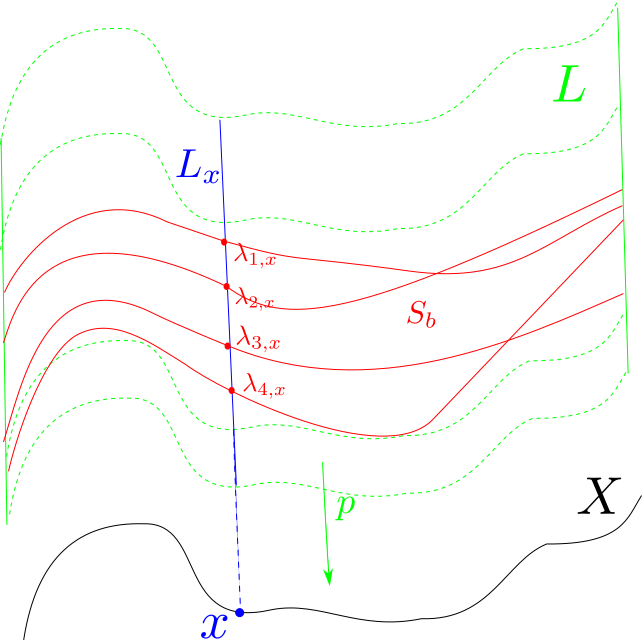
\includegraphics[width=0.5\textwidth]{curvaespectral.png}
	 \caption{The spectral curve on its ambient space $L$. The elements $\left\{ \lambda_{1,x},\dots,\lambda_{4,x} \right\}$ are the ``eigenvalues'' of $\varphi_x$.}
	 \label{fig:spectral}
       \end{figure}

       \begin{prop}
	 Assume that $L^n$ is base point free. Then, for generic elements $b\in \bigoplus_{i=1}^n H^0(X,L^i)$, the spectral curve $S_b$ is smooth.
       \end{prop}

       \begin{proof}
	 The spectral curve $S_b$ is an irreducible hypersurface of $L$, so it can be thought as a divisor on it and on its compactification $\PP(L\oplus \OO_X)$. Moreover, as the $b$ varies, $s_b$ defines a linear subspace of $\PP(H^0(L,p^*L^n))$, so 
	 \begin{equation*}
	   \mathfrak{d}=\left\{ S_b: b\in \bigoplus_{i=1}^n H^0(X,L^i) \right\}
	 \end{equation*}
	 is a linear system of divisors on $L$. Bertini's theorem says that, away from the base locus of $\mathfrak{d}$, the generic divisor of the system is smooth. Let us check then that the base locus of $\mathfrak{d}$ is empty.

	 Suppose that $y \in L$ is a base point of $\mathfrak{d}$. Then, since $(\lambda^n)_0 \in \mathfrak{d}$, $\lambda(y)=0$. But then $s_b(y)=p^*b_n(y)=b_n(p(y))$ for every $b$ and, since $y$ is a base point, $s_b(y)=0$. Therefore $b_n(p(y)) = 0$ for every $b_n \in H^0(X,L^n)$, so $p(y)$ is a base point of $L^n$. But by hypothesis $L^n$ is base point free, so we reach a contradiction.
       \end{proof}

       Note now that the restriction of the natural projection $p:L\rightarrow X$ defines a map,
       \begin{center}
	 \begin{tikzcd}
	   S_b	   \arrow[hook]{rr}\arrow{rrdd}[anchor=north,rotate=-30]{\pi} && L\arrow{dd}[anchor=west]{p} \\ 
	    && \\
	    && X.
	  \end{tikzcd}
	\end{center}
	Since $\pi:S_b\rightarrow X$ is a morphism of Riemann surfaces it defines a branched covering of $S_b$ over $X$. Note that at a point $x$ where this morphism is étale the fiber has exactly $n$ points, the $n$ eigenvalues of $\varphi_x$. Therefore the degree of the map $\pi$ is $\deg \pi = n$. Similarly, the \emph{branch locus} will be given precisely by those points $x\in X$ where some eigenvalues of $\varphi_x$ have algebraic multiplicity $>1$. By the same reason, the \emph{ramification divisor} $R$ on $S_b$ is defined as the zero divisor of $\Disc(s_b)\in H^0(X,p^*L^{n(n-1)})$, which is the discriminant of $s_b$, or equivalently, the resultant of $s_b$ and its derivative
	\begin{equation*}
	  \Disc(s_b)=\Res\left(s_b, \frac{\partial}{\partial \lambda} s_b\right).
	\end{equation*}
	$R$ is the zero locus of a section of $p^*L^{n(n-1)}$, so its degree is precisely
	\begin{equation*}
	  \deg R = \deg (L^{n(n-1)})=n(n-1)\deg L.
	\end{equation*}
	The Riemann-Hurwitz formula yields the genus of the spectral curve,
	\begin{equation*}
	  2g_{S_b} - 2 = n(2g-2) + \deg R = n(2g-2) + n(n-1)\deg L,
	\end{equation*}
	\begin{equation*}
	  g_{S_b}= 1+n(g-1)+ \frac{n(n-1)}{2}\deg L.
	\end{equation*}

	We are now in position to prove the spectral correspondence:
	\begin{thm}[Beauville-Narasimhan-Ramanan, \cite{bnr}]
	  Take $b \in \bigoplus_{i=1}^n H^0(X,L^i)$ such that the spectral curve $S_b$ is irreducible and smooth. We have a bijective correspondence, up to isomorphism, between holomorphic line bundles over $S_b$ of degree $\delta$ and pairs $(\ve{E},\varphi)$, where $\ve{E}$ is a holomorphic vector bundle over $X$ of rank $n$ and degree $d$, and $\varphi$ is a $L$-twisted endomorphism with characteristic polynomial
	  \begin{equation*}
	    P_\varphi(T)=P_b(T):=T^n + \sum_{i=1}^n b_i T^{n-i}.   
	  \end{equation*}
	  The degrees $d$ and $\delta$ are related by
	  \begin{equation*}
	    d=\delta - \frac{n(n-1)}{2}\deg L .
	  \end{equation*}
	\end{thm}

	\begin{proof}
	  Let $M$ be a holomorphic line bundle over $S_b$ of degree $\delta$. We can consider the direct image bundle $\pi_*M$, which is a rank $\deg \pi=n$ vector bundle over $X$ and its degree is given by the formula
	  \begin{equation*}
	    \deg(\pi_*M)=\deg M + (1-g_{S_b}) - \deg \pi (1-g)=\delta -  \frac{n(n-1)}{2}\deg L.
	  \end{equation*}
	  Let now $U\subset X$ be any open subset. If we take tensor product by the tautological section restricted to $\pi^{-1}(U)$, $\lambda|_{\pi^{-1}(U)} \in H^0(\pi^{-1}(U),\pi^*L)$ we can construct a homomorphism
	  \begin{equation*}
	    \otimes \lambda|_{\pi^{-1}(U)}: H^0(\pi^{-1}(U),M) \rightarrow H^0(\pi^{-1}(U),M \otimes \pi^*L).
	  \end{equation*}
	  But, by definition of the direct image sheaf,
	  \begin{equation*}
	    H^0(\pi^{-1}(U),M)=H^0(U,\pi_*M),
	  \end{equation*}
	  \begin{equation*}
	    H^0(\pi^{-1}(U),M\otimes \pi^{*}L)=H^0(U,\pi_*(M\otimes \pi^*L))=H^0(U,\pi_*M \otimes L).
	  \end{equation*}
	  This gives a homomorphism of locally free sheaves
	  \begin{equation*}
	      \OO(\pi_*M) \rightarrow \OO(\pi_*M \otimes L),
	  \end{equation*}
	  that induces a $L$-twisted endomorphism
	  \begin{equation*}
	    \varphi:\pi_*M \rightarrow \pi_*M\otimes L.
	  \end{equation*}
	  Moreover, by construction $P_b(\varphi)=0$, and since $P_b$ is irreducible, the Cayley-Hamilton theorem guarantees that $P_b$ is the characteristic polynomial of $\varphi$.

	  On the other hand, take a pair $(\ve{E},\varphi)$, with $\ve{E}$ a rank $n$ holomorphic vector bundle and $\varphi$ a $L$-twisted endomorphism such that $b=(\sigma_1(\varphi),\dots,\sigma_n(\varphi))$. Consider the pullback bundle $\pi^*\ve{E}$,
	  \begin{center}
	    \begin{tikzcd}
	      \pi^*\ve{E}	      \arrow{rr}\arrow{dd} && \ve{E}\arrow{dd} \\ 
	       && \\
	       S_b\arrow{rr}[anchor=south]{\pi} && X.
	     \end{tikzcd}
	   \end{center}
	   The pullback section $\pi^*\varphi\in H^0(S_b,\End (\pi^*\ve{E})\otimes \pi^*L)$ must satisfy
	   \begin{equation*}
	     P_{\pi^*\varphi}(\lambda|_{S_b})=(\lambda|_{S_b})^n+ \sum_{i=1}^n \pi^*b_i (\lambda|_{S_b})^{n-i} = s_b|_{S_b}=0,
	   \end{equation*}
	   since $S_b=(s_b)_0$. Therefore, locally we can see $\lambda$ as an eigenvalue of $\varphi$ and one could construct the line bundle $M$, at least away from the ramification divisor, as the bundle defined at each point $x$ by the eigenspace of $\varphi_x$ associated to $\lambda_x$. Globally what we do is consider $\lambda|_{S_b}\id - \pi^*\varphi$ as a morphism of locally free sheaves and the sheaf $\ker(\lambda|_{S_b}\id - \pi^*\varphi) \subset \pi^*\ve{E}$, which is a rank one locally free sheaf, so it defines a line bundle $M$ over $S_b$ such that $\pi_*M \cong\ve{E}$. Another direct way to do this is to define $M$ by the exact sequence
	   \begin{center}
	     \begin{tikzcd}
	       0 \arrow{r} & M(-R) \arrow{r} & \pi^*\ve{E} \arrow{rr}{\lambda|_{S_b}\id -\pi^*\varphi} && \pi^*(\ve{E}\otimes L) \arrow{r} & M\otimes \pi^*L  \arrow{r} & 0.
	     \end{tikzcd}
	   \end{center}
	\end{proof}

	\section{Hitchin's equations}
	Let us now apply the results of the previous section to the case of the Hitchin system
	\begin{align*}
	  H:T^*\Bun(n,d)& \longrightarrow \BB = \bigoplus_{i=1}^n H^0(X,K_X^i) \\
	  (\ve{E},\varphi) &\longmapsto (\sigma_1(\varphi),\dots,\sigma_n(\varphi)). 
	  \end{align*}
	  The fiber of some point $b=(b_1,\dots,b_n)\in \BB$ by this map is formed precisely by (isomorphism classes of) that pairs $(\ve{E},\varphi)$ such that $\ve{E}$ is a holomorphic \textit{stable} vector bundle of rank $n$ and degree $d$ and $\varphi:\ve{E}\rightarrow \ve{E}\otimes K_X$ is a $K_X$-twisted endomorphism with $P_\varphi(T)=P_b(T)$. Moreover, $K_X^n$ is base point free, so for generic $b\in \BB$ the spectral curve $S_b$ will be irreducible and smooth. Stability is an open condition, so in this case the Beauville-Narasimhan-Ramanan theorem says that the fiber of a generic $b$ is an open subset of the set of isomorphism classes of holomorphic line bundles over $S_b$ of degree 
	  $$\delta=d+\frac{n(n-1)}{2}\deg K_X=d+n(n-1)(g-1).$$
	  But this set of isomorphism classes is precisely the component $\Pic^\delta (S_b)$ of the Picard group, which is isomorphic to the Jacobian $J(S_b)$; so it is indeed a complex torus! Moreover, the dimension of this complex torus is the genus of the spectral curve, and if we compute it the \textit{miracle} occurs:
	  \begin{equation*}
	    g_{S_b}=1+n(g-1)+\frac{n(n-1)}{2}\deg K_X=1+n^2(g-1).
	  \end{equation*}
	  Summing up, we have proven that for some point $b\in \BB$, the fiber of the Hitchin map $H^{-1}(b)$ is an open set of $\Pic^{\delta}(S_b)$, a complex torus of dimension $n^2(g-1)+1$. This completes the proof of Hitchin's theorem \ref{hitchinsystem}.

	  A natural question to ask now is what happens to the remaining elements of the Jacobian: if they do not yield elements of $T^*\Bun(n,d)$, what do they correspond to? This suggest the existence of a wider symplectic manifold, of which $T^*\Bun(n,d)$ is a subset. 

	  Recall that we constructed the space $T^*\Bun(n,d)$ by fixing a smooth vector bundle $E$ of rank $n$ and degree $d$ over $X$ and considering the action of $\GG^c$ on the space $\AA^c=\AA_{\delbar}^s \times \Omega^{1,0}(X,\End E)$. To get this wider space we will now consider the action of the real group $\GG$ on the space $\AA_h \times \Omega^{1,0}(X,\End E)$. Of course, to do this we first have to fix an Hermitian metric $h$ on $E$. We then get a symplectic structure on $\AA_h \times \Omega^{1,0}(X,\End E)$ given by
	  \begin{equation*}
	    \omega\left( (A_1,\varphi_1),(A_2,\varphi_2) \right)=-\int_X \tr(A_1\wedge A_2) +2i\ \mathrm{Im}\ \tr(\varphi_1 \varphi_2^\dagger),
	  \end{equation*}
	  where $A_i \in \Omega^{1}(X,\mathfrak{u}_h(E))$ and $\varphi_i \in \Omega^{1,0}(X,\End E)$.

	  \begin{rem}\label{obsproducto}
	    Let us see explicitly what we mean by $\varphi_1\varphi_2^\dagger$. $\varphi$ is an element of $\Omega^{1,0}(X,\End E)=\Gamma(\Lambda^{1,0}(X)\otimes\End E)$, thus, locally it can be seen as $\varphi=\phi \otimes \alpha$, with $\phi: X \rightarrow \End E$ and $\alpha:X\rightarrow \Lambda^{1,0}(X)$. By $\varphi^\dagger$ then we mean an element of $\Omega^{0,1}(X,\End E)$ which locally looks like $\varphi^\dagger=\phi^{\dagger} \otimes \bar{\alpha}$ with $\phi^{\dagger}$ the transpose conjugate (globally the adjoint, given by $h$) of $\phi$ and $\bar{\alpha}:X\rightarrow \Lambda^{0,1}(X)$ the conjugate of $\alpha$. By $\varphi_1 \varphi_2^\dagger$ we mean an element of $\Omega^{1,1}(X,\End E)$, which locally looks like
	    \begin{equation*}
	      \varphi_1 \varphi_2^\dagger=(\phi_1\phi_2^{\dagger})\otimes \alpha_1 \wedge \bar{\alpha}_2.
	    \end{equation*}
	    We can also consider elements of the form
	    \begin{equation*}
	      [\varphi_1, \varphi_2] := \varphi_1 \varphi_2 + \varphi_2 \varphi_1 = (\phi_1\phi_2)\otimes \alpha_1 \wedge \alpha_2 + (\phi_2 \phi_1) \otimes \alpha_2 \wedge \alpha_1=[\phi_1,\phi_2] \otimes \alpha_1 \wedge \alpha_2.
	    \end{equation*}
	  \end{rem}
	  
	  Remember that the elements $g$ of the group $\GG$ act by conjugation $(\nabla,\varphi)\mapsto (g\nabla g^{-1},g\varphi g^{-1})$. 
	  \begin{prop}
	    The action of $\GG$ on $\AA_h\times \Omega^{1,0}(X,\End E)$ admits a momentum map,
	  \begin{equation*}
	    \mu(\nabla,\varphi)=-F-[\varphi,\varphi^\dagger]-2\pi i \mu(E) \id_E \omega_X.
	  \end{equation*}
	  \end{prop}
	  \begin{proof}
	    The part of the momentum map corresponding to $-F-2\pi i \mu(E) \id_E \omega_X$ comes form the action on $\AA_h$ and the proof is identical to the case of the previous chapter. 
	    
	    On the other hand, taking into account the previous remark we can we can focus in computing the momentum map for a much simpler case:
	    \begin{lema}
	    Consider the space $\End\ \CC^n$ equipped with the symplectic form
	    \begin{equation*}
	      \omega(A,B)=-\mathrm{Im}\ \tr(AB^{\dagger}),
	    \end{equation*}
	    and consider the action of $\UU(n)$ on it by conjugation. This action admits a momentum map
	    \begin{equation*}
	      \mu(A)= \tfrac{i}{2} [A,A^{\dagger}].
	    \end{equation*}
	    \end{lema}
	    \begin{proof}
	      First of all, notice that we can identify $\uu(n)$ with its dual via the pairing
	      \begin{equation*}
		\esc{H,K}=\tr(HK^\dagger)=-\tr(HK).
	      \end{equation*}
	      The Lie algebra $\uu(n)$ is formed by skew-Hermitian matrices, so
	      \begin{equation*}
		\overline{\esc{H,K}}=\tr(KH^\dagger)=\tr\left( (-K^\dagger)(-H) \right)=\tr (K^\dagger H) =\tr (HK^\dagger ) = \esc{H,K}.
	      \end{equation*}
	      That is, $\esc{H,K}$ is indeed a real number. Also notice that 
	      \begin{equation*}
		\mu(A)^{\dagger}=-\tfrac{i}{2}[A,A^{\dagger}]=-\mu(A),
	      \end{equation*}
	      so $\mu(A) \in \uu(n)$; the momentum map is well defined.
	      
	      To see how $\vec{H}$ looks like for an element $H\in \mathfrak{u}(n)$, just compute
	      \begin{equation*}
		\vec{H}(A)=\left.\frac{d}{dt} \right|_{t=0} (e^{Ht}Ae^{-Ht})=HA-AH=[H,A].
	      \end{equation*}
	      Let us compute also $d_{A}\mu(B)$ for some $B \in \End \CC^n$
	      \begin{equation*}
		d_A \mu(B) =\left.\frac{d}{dt} \right|_{t=0} \mu(A+tB)=\tfrac{i}{2}\left.\frac{d}{dt} \right|_{t=0}    [A+tB,A^{\dagger}+tB^\dagger]=\tfrac{i}{2} \left([B,A^{\dagger}] + [A,B^{\dagger}]\right).
	      \end{equation*}
	      Now
	      \begin{equation*}
		\esc{d_A\mu(B),H}=-\tfrac{i}{2} \tr([B,A^\dagger]H+[A,B^{\dagger}]H)
	      \end{equation*}
	      Using the cyclic property of the trace and the fact that $H^\dagger=-H$  one gets
	      \begin{equation*}
		\tr([A,B^\dagger]H)=\tr(H[A,B^\dagger])-\tr(H^\dagger[A,B^\dagger])=-\overline{\tr([B,A^\dagger]H)}.
	      \end{equation*}
Therefore
	      \begin{equation*}
		\esc{d_A\mu(B),H}=- \tfrac{i}{2}2i \mathrm{Im}\ \tr([B,A^\dagger]H)=  \mathrm{Im}\ \tr([B,A^\dagger]H).
	      \end{equation*}
	      On the other hand
	      \begin{equation*}
		\omega(B,\vec{H}(A))=-\mathrm{Im}\ \tr(B[A^\dagger,H^\dagger])=\mathrm{Im}\ \tr([B,A^\dagger]H])=\esc{d_A\mu(B),H}.
	      \end{equation*}
	      This finishes the proof of the lemma.
	    \end{proof}
	    In the general case, the symplectic structure locally has the form
	    \begin{equation*}
	    \omega(\varphi_1,\varphi_2)=-2i \int_X \mathrm{Im}\  \tr(\varphi_1\varphi_2^\dagger)=-2i \int_X \mathrm{Im}\ [\tr(\phi_1\phi_2^\dagger)] \otimes \alpha_1 \wedge \bar{\alpha_2}.
	    \end{equation*}
	    Therefore, the momentum map must have the form
	    \begin{equation*}
	      \mu(\varphi)=-[\varphi,\varphi^\dagger] \in \Omega^2(\uu_h(E)).
	    \end{equation*}
	    This finishes the proof of the proposition.
	  \end{proof}

	  Now that we have a momentum map, and assuming that the $\GG$-action verifies all the technical requirements, we can take the symplectic quotient $\mu^{-1}(0)/\GG$. Let us consider now the subvariety
	  \begin{equation*}
	    \left\{ (\nabla,\varphi) \in \AA_h \times \Omega^{1,0}(X,\End E) : \nabla^{0,1}\varphi = 0\right\}.
	  \end{equation*}
	  By avoiding possible singularities, this variety inherits the symplectic structure from $\AA_h\times \Omega^{1,0}(X,\End E)$ and, since it is $\GG$-invariant, we can use the restriction of the momentum map to take another symplectic quotient.
	  The space we obtain is the \emph{moduli space of solutions to the Hitchin equations} on $E$, that is, the set of equivalence classes of pairs $(\nabla,\varphi) \in \AA_h \times \Omega^{1,0}(X,\End\ E)$ that satisfy \emph{Hitchin's equations}:
	  \begin{equation*}
	    \begin{cases}
	      F+[\varphi,\varphi^\dagger]=-2\pi i \mu(E) \id_E \omega_X, \\
	      \nabla^{0,1}\varphi=0.
	    \end{cases}
	  \end{equation*}
	  
	  In the next section we are going to see how this space corresponds to a broader notion of stability for pairs $(\ve{E},\varphi)$, with $\ve{E}$ a holomorphic vector bundle and $\varphi:\ve{E}\rightarrow \ve{E}\otimes K_X$ a $K_X$-twisted endomorphism and we will show that this moduli space is precisely the wider symplectic manifold containing $T^*\Bun(n,d)$ and the pairs associated to the remaining points of the Jacobian in the spectral correspondence.

	  \section{Higgs bundles}
	  \begin{defn}
	    A pair $(\nabla,\varphi) \in \AA_h \times \Omega^{1,0}(X,\End\ E)$ is called \emph{irreducible} if there exist no subbundles $E'\subset E$ which are preserved by both $\nabla$ and $\varphi$. 
	  \end{defn}
	  \begin{thm}[Hitchin correspondence] \label{Hitchin correspondence}
	    Let $(E,h)$ be a Hermitian complex vector bundle of rank $n$ and degree $d$ on a compact Riemann surface $X$.
	    An irreducible pair $(\nabla ,\varphi) \in \AA_h \times \Omega^{1,0}(X,\End\ E)$ is a solution to the Hitchin equations if and only if for every proper subbundle $E'\subset E$ which is invariant by $\nabla^{0,1}$ and $\varphi$,
	    \begin{equation*}
	      \mu(E')<\mu(E).
	    \end{equation*}
	  \end{thm}
	  The proof of this theorem uses the same techniques and is very similar to the proof of Theorem \ref{narasimhanseshadri}. As in that case, we will only prove the ``easy'' direction of the equivalence.
	  \begin{proof}
	    Let $(\nabla,\varphi)$ be a solution of the Hitchin equations
	  \begin{equation*}
	    \begin{cases}
	      F+[\varphi,\varphi^\dagger]=-2\pi i \mu(E) \id_E \omega_X, \\
	      \nabla^{0,1}\varphi=0.
	    \end{cases}
	  \end{equation*}
	  and define $\delbar_{\ve{E}}=\nabla^{0,1}$. Let $E'\subset E$ be a subbundle preserved by $\delbar_{\ve{E}}$ such that $\varphi(E')\subset E'\otimes K_X$. The Hermitian metric gives a smooth splitting $E=E'\oplus E''$, and we can write
	  \begin{equation*}
	    \varphi=
	    \left(
	    \begin{array}{cc}
	      \varphi_{E'} & \theta \\
	      0 & \varphi_{E''}
	    \end{array}
	    \right),
	  \end{equation*}
	  for $\theta \in \Omega^{1,0}(X,\Hom(E'',E'))$.
	  The top left element of $[\varphi,\varphi^\dagger]$ is
	  \begin{equation*}
	    \varphi_{E'}\varphi_{E'}^\dagger + \theta\theta^\dagger - \varphi_{E'}^\dagger\varphi_{E'}=[\varphi_{E'},\varphi_{E'}^\dagger] + \theta  \theta^\dagger.
	  \end{equation*}
	  Using the equation
	  \begin{equation*}
  F=\left(
  \begin{array}{cc}
    F_{E'}-\beta\beta^\dagger & \nabla_{\Hom(E'',E')}\beta \\
    -\nabla_{\Hom (E',E'')}\beta^\dagger & F_{E''}-\beta^\dagger \beta
  \end{array}\right),
	  \end{equation*}
	  from the proof of Narasimhan-Seshadri (Theorem \ref{narasimhanseshadri}) we have
	  \begin{equation*}
	    F_{E'}-\beta \beta^{\dagger} + [\varphi_{E'},\varphi_{E'}^\dagger]+\theta \theta^{\dagger}=-2\pi i \frac{d}{n}\id_{E'} \omega_X.
	  \end{equation*}
	  Now, since $\tr[\varphi,\varphi^\dagger]=0$, taking the trace and integrating we get
	  \begin{equation*}
	    \frac{i}{2\pi}\int_X \tr F_{E'} + \norm{\beta}^2 + \norm{\theta}^2  = \mu(E) \rk E',
	  \end{equation*}
	  and hence
	  \begin{equation*}
	   \mu(E')= \deg E'/\rk E'= \mu(E)-\norm{\beta}^2 - \norm{\theta}^2.
	  \end{equation*}
	  Since the pair $(\nabla,\varphi)$ is irreducible, $\norm{\beta}$ and $\norm{\theta}$ are nonzero, so $\mu(E')<\mu(E)$.
	  \end{proof}

	  \begin{defn}
	    Let $X$ be a compact Riemann surface. A \emph{Higgs bundle} (or \emph{Hitchin pair}) over $X$ is a pair $(\ve{E},\varphi)$, where $\ve{E}$ is a holomorphic vector bundle over $X$ and $\varphi:\ve{E}\rightarrow \ve{E}\otimes K_X$ is a $K_X$-twisted endomorphism.
	    A Higgs bundle $(\ve{E},\varphi)$ is said to be \emph{stable} if for every proper holomorphic subbundle $\ve{E}' \subset \ve{E}$ such that $\varphi(\ve{E}')\subset \ve{E}'\otimes K_X$
	    \begin{equation*}
	      \mu(\ve{E}')<\mu(\ve{E}).
	    \end{equation*}
	    The \emph{moduli space of stable Higgs bundles of rank $n$ and degree $d$}, $\Hig(n,d)$, is defined as the set of isomorphism classes of stable Higgs bundles $(\ve{E},\varphi)$ with $\rk\ \ve{E}=n$ and $\deg \ve{E}=d$.
	  \end{defn}

	  In \cite{hitchinselfduality}, Hitchin gave an analytic construction of a particular case of rank $2$ of this moduli space and a general GIT construction was given by Nitsure in \cite{nitsure}.
	  \begin{thm}\label{thm:higgs}
	    The moduli space $\Hig(n,d)$ is a complex manifold of dimension $2+2n^2(g-1)$, where $g$ is the genus of $X$.
	  \end{thm}

	  The Hitchin correspondence \ref{Hitchin correspondence} can be now reinterpreted as follows
	  \begin{corol}
	    Let $(E,h)$ be a smooth Hermitian vector bundle of rank $n$ and degree $d$. The moduli space of solutions to the Hitchin equations on $E$ is homeomorphic to the moduli space of stable Higgs bundles $\Hig(n,d)$.
	  \end{corol}

	  We can now extend the Hitchin map to the bigger space $\Hig(n,d)\supset T^*\Bun(n,d)$,
	  \begin{align*}
	    H :\Hig(n,d)&\longrightarrow \BB=\bigoplus_{i=1}^n H^0(X,K^i_X)\\ 
	    (\ve{E},\varphi) &\longmapsto (\sigma_1(\varphi),\dots,\sigma_n(\varphi)). 
	    \end{align*}
	    Take now a point $b\in \BB$ such that the spectral curve $S_b$ is irreducible and smooth. For every holomorphic line bundle $M$ over $S_b$ the spectral correspondence gives us a Higgs bundle $(\ve{E}=\pi_*M, \varphi)$. 
	    \begin{prop}
	      The pair $(\ve{E},\varphi)$ induced by a line bundle $M$ on an irreducible spectral curve $S_b$ is stable.
	    \end{prop}
	    \begin{proof}
	      Suppose that $\ve{E}'\subset \ve{E}$ is a proper holomorphic subbundle invariant by $\varphi$. Then we can take the characteristic polynomial of $\varphi|_{\ve{E}'}$ and it must divide the characteristic polynomial of $\varphi$, thus contradicting that the spectral curve is irreducible.
	    \end{proof}

	    As a conclusion, we get that generic fibers of the Hitchin map $H:\Hig(n,d) \rightarrow \BB$ are whole Jacobians of the spectral curve

	    \section{Deformations of Higgs bundles}
	    In this section we are going to compute the dimension of $\Hig(n,d)$, stated in Theorem \ref{thm:higgs}, using deformation theory. As in the case for vector bundles, the idea is to identify the tangent space of $\Hig(n,d)$ at some point $(\delbar_{\ve{E}},\varphi)$ and find its dimension.

	    First of all, note that an analytic construction of $\Hig(n,d)$ can be given if we consider the variety
	    \begin{equation*}
	     \HH= \left\{(\delbar_{\ve{E}},\varphi) \in\AA^s_\partial \times \Omega^{1,0}(X,\End E) : \delbar_{\ve{E}}\varphi=0 \right\}
	    \end{equation*}
	    and its open subset
	    \begin{equation*}
	      \HH^s=\left\{ (\delbar_{\ve{E}},\varphi) \in \HH : (\delbar_{\ve{E}},\varphi) \text{ is stable} \right\}      .
	    \end{equation*}
	    As usual, an element $g$ of the complex group $\GG^c=\Gamma(\Aut E)$ acts on $\HH$ by conjugation,
	    \begin{equation*}
	      (\delbar_{\ve{E}},\varphi) \mapsto (g\delbar_{\ve{E}}g^{-1},g\varphi g^{-1}).
	    \end{equation*}
	    We can then obtain the moduli space of Higgs bundles as the quotient $\Hig(n,d)=\HH^s/\GG^c$, where $n=\rk\ E$ and $d= \deg E$.

	    The differential of action of the complex group on $\HH$ is a mapping from the Lie algebra $\Lie \GG^c= \Gamma(\End\ E)$ to the tangent space of $\HH$,
	    \begin{align*}
	      f:\Gamma(\End\ E)&\longrightarrow T_{(E,\varphi)}\HH\\ 
	      \xi &\longmapsto (\delbar_{\ve{E}} \xi, [\varphi,\xi]). 
	      \end{align*}
	      Since stability is an open condition, we can identify the tangent space to the moduli space with the quotient of the tangent space of $\HH$ by the image of this mapping, $$T_{(\delbar_{\ve{E}},\varphi)}\Hig(n,d)=T_{(\delbar_{\ve{E}},\varphi)}\HH/\im f.$$ On the other hand, to obtain how an element of the tangent space $T_{(\delbar_{\ve{E}},\varphi)}\HH$ looks like, consider a small perturbation $$(\delbar_{\ve{E}}(\epsilon), \varphi(\epsilon))=(\delbar_{\ve{E}}+\epsilon A, \varphi + \epsilon \psi),$$ for $(A,\psi) \in \Omega^{0,1}(X,\End \ E) \oplus \Omega^{1,0}(X, \End \ E)$ and impose that the condition $\delbar_{\ve{E}}(\epsilon)\varphi(\epsilon)=0$ is infinitesimally satisfied. That is,
	    \begin{equation*}
	      0=\left.\frac{d}{d\epsilon} \right|_{\epsilon=0} \delbar_{\ve{E}}(\epsilon)\varphi(\epsilon)=\left.\frac{d}{d\epsilon} \right|_{\epsilon=0}\left[ \delbar_{\ve{E}} \varphi + \epsilon\left( [A,\varphi]+\delbar_{\ve{E}}\psi \right)+ o(\epsilon^2) \right] = [A,\varphi]+\delbar_{\ve{E}}\psi.
	    \end{equation*}
	    Therefore, we can think of $T_{(\delbar_{\ve{E}},\varphi)}\HH$ as the kernel of the map
	    \begin{align*}
	      g :\Omega^{0,1}(X,\End \ E) \oplus \Omega^{1,0}(X, \End \ E)&\longrightarrow \Omega^{1,1}(X, \End\ E)\\ 
	      (A,\psi) &\longmapsto [A,\varphi]+\delbar_{\ve{E}}\psi. 
	      \end{align*}
	      Note then that $f$ is well defined,
	      \begin{equation*}
		g\circ f(\xi)=[\delbar_{\ve{E}}\xi,\varphi]+\delbar_{\ve{E}}[\varphi,\xi]=[\delbar_{\ve{E}}\xi,\varphi]+[\delbar_{\ve{E}}\varphi,\xi]-[\delbar_{\ve{E}}\xi,\varphi]=0,
	      \end{equation*}
	      since $\delbar_{\ve{E}}\varphi=0$. In other words, what we are saying is that we have a chain complex
	      \begin{center}
		\begin{tikzcd}
		  C^\bullet: \Gamma(\End\ E) \arrow{r}{f}&  \Omega^{0,1}(X,\End \ E) \oplus \Omega^{1,0}(X, \End \ E) \arrow{r}{g}& \Omega^{1,1}(X,\End\ E)
		\end{tikzcd}
	      \end{center}
	      and the tangent space $T_{(\delbar_{\ve{E}},\varphi)}\Hig(n,d)$ is the first cohomology of this complex, $H^1(C^\bullet)$.

	      Consider now the double complex
	      \begin{center}
		\begin{tikzcd}
		   0 \arrow{r}\arrow{d} & \Gamma(\End\ E) \arrow{r}{=}\arrow{d}{f} &\Gamma(\End\ E) \arrow{d}{\delbar_{\ve{E}}} 		  \\ 
		  \Omega^0(X,\End\ E \otimes K_X) \arrow{d}{\delbar_{\ve{E}}} \arrow[hook]{r}{\iota} & \Omega^{0,1}(X,\End\ E)  \oplus \Omega^{1,0}(X, \End\ E) \arrow{d}{g}\arrow{r}{\pr_1} & \Omega^{0,1}(X,\End\ E) \arrow{d}{\delbar_{\ve{E}}} \\
		  \Omega^{0,1}(X,\End\ E \otimes K_X) \arrow{d}{\delbar_{\ve{E}}}\arrow{r} & \Omega^{1,1}(X, \End\ E) \arrow{r} & 0 \\
		  0.
		\end{tikzcd}
	      \end{center}
	      The rows of this complex are short exact sequences so we get a short exact sequence of complexes
	      \begin{center}
		\begin{tikzcd}
		  0 \arrow{r} & \Omega^{0,\bullet}(X,\End\ E \otimes K_X)[1] \arrow{r} & C^\bullet \arrow{r}& \Omega^{0,\bullet}(X,\End\ E) \arrow{r} & 0,
		\end{tikzcd}
	      \end{center}
	      where the $[1]$ after a complex denotes shifting one place and adding zero in the first place. This induces a long exact sequence in cohomology
	      \begin{align*}
		  0 \rightarrow  H^0(C^\bullet) \rightarrow  H^0(X,\End\ E) \rightarrow H^0(X,\End\ E \otimes K_X) \rightarrow &		  \\ 
		  \rightarrow H^1(C^\bullet) \rightarrow H^1(X, \End\ E) \rightarrow H^1(X, \End\ E \otimes K_X) \rightarrow H^2(C^\bullet) \rightarrow 0.
	      \end{align*}
	      The Euler characteristic of any exact sequence vanishes, so

	      \begin{equation*}
		H^0(C^\bullet) - H^1(C^\bullet) + H^2(C^\bullet) - \chi(\End\ E) + \chi(\End\ E \otimes K_X)=0.
	      \end{equation*}
	      Now, note that $\chi(\End\ E)= -\chi(\End\ E \otimes K_X)$ and recall that we computed that $\chi(\End\ E)= n^2(1-g)$. 
	      Therefore
	      \begin{equation*}
		\dim H^1(C^\bullet)= \dim H^0(C^\bullet) + \dim H^2(C^\bullet) + 2n^2(g-1).
	      \end{equation*}

	      Noting that, by Serre duality
	      \begin{align*}
		H^1(X,\End\ E)^*\cong H^0(X,(\End E)^* \otimes K_X) \cong H^0(X,\End E \otimes K_X) \\
		H^1(X,\End\ E \otimes K_X)^* \cong H^0(X,(\End\ E \otimes K_X)^*\otimes K_X) \cong H^0(X, \End\ E),
	      \end{align*}
	      we can dualize in the above exact sequence and we get that $H^2(C^\bullet)^*\cong H^0(C^\bullet)$, so $$\dim H^2(C^\bullet)=\dim H^0(C^\bullet).$$ 
	      To find this dimension we use the following result:
	      \begin{prop}
		If $(\ve{E},\varphi)$ is a stable Higgs bundle, then 
		\begin{equation*}
		  H^0(C^\bullet) = \CC.
		\end{equation*}
	      \end{prop}
	      \begin{proof}
	Note that 
	\begin{equation*}
	  H^0(C^\bullet)=\ker f = \left\{ \xi \in H^0(X,\End\ \ve{E}): [\varphi,\xi]=0 \right\}.
	\end{equation*}
	What we are going to prove is that every endomorphism $\xi$ that satisfies that condition is a multiple of the identity $\id_{\ve{E}}$. Indeed, let $\lambda \in \CC$ be an eigenvalue of $\xi_x:\ve{E}_x \rightarrow \ve{E}_x$ and define the endomorphism $\eta= \xi-\lambda \id_{\ve{E}}$. Since $\lambda$ is an eigenvalue of $\xi_x$, we have $\det \eta_x=0$. Assuming that $\eta$ is nonzero, we will prove that $\eta$ is injective and hence $\det \eta_x \neq 0$ arriving at a contradiction. To see this, suppose that $\im \eta \subset \ve{E}$ is a holomorphic strict subbundle of $\ve{E}$. Note too that $\im \eta$ is $\varphi$-invariant, since, if $w=\eta(v)$, then $$\varphi(w)=\varphi((\xi - \lambda \id_{\ve{E}})(v))= \varphi(\xi(v)) -  \varphi(\lambda v)=\xi(\varphi(v))-\lambda \varphi(v)=\eta(\varphi(v)),$$
	since $[\varphi,\xi]=0$. Therefore, since $(\ve{E},\varphi)$ is stable, $\mu(\im \eta) < \mu(\ve{E})$. But we also have that $\mu(\ve{E})<\mu(\im \eta)$, so $\mu(\ve{E})<\mu(\ve{E})$ and we have a contradiction. Therefore $\eta$ is injective. We conclude then that $\eta=0$, so $\xi=\lambda \id_{\ve{E}}$.
	      \end{proof}

	      In conclusion, we get that $\dim H^2(C^\bullet)=\dim H^0(C^\bullet)=1$. We then arrive at the result we were looking for:
	      \begin{equation*}
		\dim \Hig(n,d)=\dim H^1(C^\bullet)=2+2n^2(g-1).
	      \end{equation*}

	      \section{An algebraic view of the spectral correspondence}
	      Up until right now we have been working in the holomorphic category, $X$ being a compact Riemann surface and working with holomorphic vector bundles on $X$. However the classical result of embedding of Riemann surfaces in projective spaces (which can be stated in modern terms as a consequence of the Kodaira embedding theorem) and the not-so-classical Serre's GAGA theorems indicate that we could aswell have worked all the time in the algebraic category. That is, we could consider $X$ to be a proyective algebraic curve and work with (algebraic) vector bundles over $X$, that is, with locally free sheaves of $\OO_X$-modules. This has been the point of view adopted by many people working in Higgs bundles, since working with the powerful tools that algebra offers can sometimes be very useful. In fact, the original paper of Beauville, Narasimhan and Ramanan $\cite{bnr}$ was written in this fashion. Let us now take a look at what we can say about the spectral correspondence from the algebraic point of view. But first consider the following example:
	      \begin{ejemplo}
		Let $V$ be a finite dimensional complex vector space and $A:V\rightarrow V$ an endomorphism. $A$ induces the following ring morphism
		\begin{align*}
		  \Phi :\CC[T]&\longrightarrow \CC[A]\subset \End V\\ 
		    p(T) &\longmapsto p(A). 
		  \end{align*}
		  This endows $V$ with the structure of a $\CC[T]$-module. Moreover, note that $\CC[A]$ is a finite $\CC$-algebra, so it must have Krull dimension $0$ and therefore discrete spectrum. Indeed, 
		  \begin{equation*}
		    \CC[A] \cong \frac{\CC[T]}{\ker \Phi}
		  \end{equation*}
		  and, by definition, $\ker \Phi$ is generated by the minimal polynomial of $A$. Since the roots of the minimal polynomial are the eigenvalues, $\Spec(\CC[A])$ consists of the eigenvalues of $A$, seen as points of the affine line $\mathbf{A}^1_\CC$.
		\qed
	      \end{ejemplo}

	      First of all, let $X$ be a complex projective smooth and irreducible curve of genus $g\geq 2$ and let $L$ be a line bundle on $X$. By an \emph{$L$-twisted Higgs bundle} we understand a pair $(E,\varphi)$, with $E$ a rank $n$ (algebraic) vector bundle on $X$ and $\varphi:E\rightarrow E\otimes L$. If we let $\LL=\Gamma(L)$ be the locally free sheaf of sections of $L$, $\varphi$ induces a sheaf morphism
	      \begin{equation*}
		\tilde{\varphi}: \Sym(\LL^{-1}) \longrightarrow \End E
	      \end{equation*}
	      in the following way. Consider a trivialization $\mathcal{U}$ of $\LL$. In some $U\subset \mathcal{U}$ we can write  $\varphi=\phi \otimes s$, with $\phi \in \Gamma(U,\End E)$ and $s\in \LL(U)$, and we have
	      \begin{equation*}
		\Sym(\LL^{-1})(U) \cong  \OO_X(U)[\lambda]=\OO_X(U) \otimes \CC[\lambda],
	      \end{equation*}
	      for $\lambda$ the dual of $s$ in $\LL^{-1}(U)=\Hom(\LL(U),\OO_X(U))$.
	      We can then define the ring homomorphism
	      \begin{align*}
		\tilde{\varphi}|_U:\OO_X(U)[\lambda]&\longrightarrow \Gamma(U,\End E)\\ 
		  p(\lambda) &\longmapsto p(\phi). 
		\end{align*}
		Globally this gives the sheaf morphism $\Sym(\LL^{-1})\rightarrow \End E$ we are looking for. Note that we can also think of the morphism $\tilde{\varphi}$ inducing a $\Sym(\LL^{-1})$-module structure on $E$.

		By definition, the total space of $L$ is the relative spectrum $\RSpec(\Sym(\LL^{-1}))$ and, if $p:L\rightarrow X$ is the bundle projection then $p_*\OO_L=\Sym(\LL^{-1})$. Since $p$ is an affine morphism, $p_*$ gives an equivalence of categories
  \begin{center}
    \begin{tikzcd}
      \left\{ \text{Quasi-coherent sheaves of } \OO_L\text{-modules} \right\}\arrow{r}{p_*} &    \left\{ \text{Quasi-coherent sheaves of } p_*\OO_L\text{-modules} \right\}      .
    \end{tikzcd}
  \end{center}
  Therefore, since the pair $(E,\varphi)$ can be seen as a $p_*\OO_L$-module, there must be a quasi-coherent sheaf $\hat{\EE}$ on $L$ such that $p_*\hat{\EE}=\EE=\Gamma(E)$. In fact, that module structure descends to a $(p_*\OO_L/\ker \tilde{\varphi})$-module structure, so the support of the sheaf $\hat{\EE}$ must be 
  \begin{equation*}
     \RSpec\left( \frac{\Sym(\LL^{-1})}{\ker \tilde{\varphi}} \right)\subset \RSpec(\Sym(\LL^{-1}))=L.
  \end{equation*}
  Note that, pointwise
  \begin{equation*}
   \left.  \frac{\Sym(\LL^{-1})}{\ker \tilde{\varphi}}\right|_x \cong \OO_{X,x} \otimes \CC[\phi(x)]
  \end{equation*}
  which has Krull dimension 1, since $\dim \OO_{X,x}=1$ and $\dim \CC[\phi(x)]=0$. Therefore, this is a $1$-dimensional scheme. For generic $\varphi$ this scheme is irreducible. In order to get an integral scheme we can consider the radical $\sqrt{\ker \tilde{\varphi}}$ and the scheme
  \begin{equation*}
    S_\varphi= \RSpec\left( \frac{\Sym(\LL^{-1})}{\sqrt{\ker \tilde{\varphi}}} \right).
  \end{equation*}

  On the other hand we can consider the coefficients of the characteristic polynomial of $\varphi$, which are sections $\sigma_i(\varphi) \in \Gamma(L^i)=\LL^i$. These sections define imbeddings 
  \begin{align*}
    \otimes \sigma_i(\varphi):\LL^{-n}&\longrightarrow \LL^{-(n-i)}.
    \end{align*}
    Locally, if $\varphi=\phi \otimes s$, $\sigma_i(\varphi)=(-1)^i s^i \tr \wedge^i \phi$, and the embedding looks like
\begin{equation*}
  \lambda^n \otimes \sigma_i(\varphi)= (-1)^i \lambda^i(s^i)  \tr \wedge^i\phi \lambda^{n-i} = \sigma_i(\phi) \lambda^{n-i}.
\end{equation*}
The sum of these imbeddings gives a homomorphism $\LL^{-n}\rightarrow \Sym(\LL^{-1})$ that locally looks like the characteristic polynomial,
    \begin{align*}
      \LL^{-n}(U)&\longrightarrow \Sym(\LL^{-1})(U)\\ 
      \lambda^n &\longmapsto \sum_{i=1}^n \sigma_i(\varphi) \otimes \lambda^n=\sum_{i=1}^n \sigma_i(\phi) \lambda^{n-i}.
      \end{align*}
      The image of this homomorphism generates an ideal sheaf $\II$ and the spectral curve can be defined as $\RSpec(\Sym(\LL^{-1})/\II)$. The Cayley-Hamilton theorem assures that $\II \subset \ker \tilde{\varphi}$. After taking the radical, the minimal and characteristic polynomial generate the same ideal and so the spectral curve coincides with the integral scheme $S_\varphi$. Moreover, away from ramification points, that is, when the characteristic polynomial of $\phi(x)$ coincides with its minimal polynomial, the rank of $\OO_{X,x}[\varphi(x)]$ as a $\OO_{X,x}$-module equals the dimension of $\CC[\varphi(x)]$ as a $\CC$-vector space, which in this case is exactly $n$. What this says is that the restriction $\pi=p|_{S_\varphi}:S_{\varphi} \rightarrow X$ is a finite morphism of degree $\deg \pi =n$.

      The spectral correspondence is now clear, $\pi$ is a finite morphism so in particular it is affine and $\pi_*$ gives an equivalence of categories
  \begin{center}
    \begin{tikzcd}
      \left\{ \text{Quasi-coherent sheaves of } \OO_{S_\varphi}\text{-modules} \right\}\arrow{r}{\pi_*} &    \left\{ \text{Quasi-coherent sheaves of } \pi_*\OO_{S_\varphi}\text{-modules} \right\}      .
    \end{tikzcd}
  \end{center}
  Of course $\pi_*\OO_{S_\varphi}=\Sym(\LL^{-1})/\ker \tilde{\varphi}$, so $\varphi$ endows $E$ with a $\pi_*\OO_{S_\varphi}$-module structure, that must correspond to a quasi-coherent sheaf $\MM$ of $\OO_{S_\varphi}$-modules such that $\pi_* \MM=\EE$. If $S_\varphi$ is smooth then the sheaf $\MM$ is locally free. Moreover, since  $\pi_*\OO_{S_\varphi}$ has the same rank, $n$, that $\EE$ as an $\OO_X$ module, $\MM$ must have rank $1$. Conversely, from a line bundle $M$ on $S_\varphi$ we recover $\pi_*M$ a rank $n$ vector bundle endowed with a $\pi_*\OO_{S_\varphi}$-module structure. 

  This point of view yields an alternative way of computing the genus of the spectral curve and the degree of the corresponding line bundle $M$ in terms of the degree $d$ of $E$. First, we can compute explicitly $\pi_*\OO_{S_\varphi}$ as
  \begin{equation*}
    \pi_*\OO_{S_\varphi}=\frac{\Sym(\LL^{-1})}{\II}=\frac{\bigoplus_{i=1}^\infty \LL^{-i}}{\langle(\sigma_1(\varphi)+\cdots+\sigma_n(\varphi))\LL^{-n}\rangle}=\bigoplus_{i=1}^{n-1} \LL^{-i}.
  \end{equation*}
  Now $\chi(S_\varphi,\OO_{S_\varphi})=\chi(X,\pi_*\OO_{S_\varphi})$, so 
  \begin{equation*}
    1-g_{S_{\varphi}}=-(\deg L)(1+\cdots+(n-1))+n(1-g)=-\deg L\frac{n(n-1)}{2}+n(1-g),
  \end{equation*}
  thus $g_{S_{\varphi}}=1+n(g-1)+\frac{n(n-1)}{2}\deg L$. To get the degree of $M$ we can use the formula (\cite[Ex. IV.2.6(a)]{hartshorne})
  \begin{equation*}
    \det \pi_*M \cong \det \pi_*\OO_{S_\varphi} \otimes \Nm_\pi M,
  \end{equation*}
  where $\Nm_\pi$ is the \emph{norm map}
  \begin{align*}
    \Nm_\pi :\Pic(S_{\varphi})&\longrightarrow \Pic(X)\\ 
    \sum_{i} n_ip_i &\longmapsto \sum_i n_i \pi(p_i). 
    \end{align*}
    Note that here we are seeing the Picard group as equivalence classes of Cartier divisors. In particular, note that $\deg M = \deg \Nm_\pi M$. Note too that
    \begin{equation*}
      \det \pi_* \OO_{S_\varphi} = \det\left( \bigoplus_{i=1}^{n-1} \LL^{-i}\right) = \LL^{-\frac{n(n-1)}{2}}.
    \end{equation*}
    Therefore
    \begin{equation*}
      d=\deg(\det \pi_*M)=\deg\left( \LL^{-\frac{n(n-1)}{2}} \right)+ \deg M= -\deg(L)\frac{n(n-1)}{2} + \deg M ,
    \end{equation*}
    so $\deg M = d+\deg(L)\frac{n(n-1)}{2}$.
	  
\section{$\SL(n,\CC)$-Higgs bundles}
The notion of a Higgs bundle can be generalized to principal bundles. In this section we will give a short example, considering principal $\SL(n,\CC)$-Higgs bundles.

\begin{defn}
  Let $G^c$ be a complex semi-simple Lie group. A $G^c$-Higgs bundle is a pair $(P,\varphi)$ where $P$ is a principal $G^c$-bundle over $X$ and the Higgs field $\varphi$ is a holomorphic section of the vector bundle $\ad P \otimes K_X$, for $\ad P$ the vector bundle associated to the adjoint representation.
\end{defn}

\begin{rem}
  When $G^c\subset \mathrm{GL}(n,\CC)$, a $G^c$-Higgs bundle is the same as a (classical) Higgs bundle of rank $n$ with some extra structure associated to $G^c$. In particular, rank $n$ classical Higgs bundles are the same as $\mathrm{GL}(n,\CC)$-Higgs bundles.
\end{rem}

When $G^c=\SL(n,\CC)$ we obtain:
\begin{defn}
  An $\SL(n,\CC)$-Higgs bundle is a Higgs bundle $(\ve{E},\varphi)$ where the rank $n$ vector bundle $\ve{E}$ has trivial determinant and the Higgs field $\varphi$ has zero trace.
\end{defn}

In this case, since $\sigma_1(\varphi)=\tr \varphi=0$, the characteristic polynomial of a $\SL(n,\CC)$-Higgs field is
\begin{equation*}
  P_\varphi(T)=T^n + \sum_{i=2}^n (-1)^i\sigma_i(\varphi) T^{n-i}.
\end{equation*}
We can consider the moduli space $\SLHig(d)$ corresponding to the subset of $\Hig(n,d)$ of $\SL(n,\CC)$-Higgs bundles. The Hitchin map restricts to this space
\begin{align*}
  H :\SLHig(d)&\longrightarrow \BB_{\SL(n,\CC)}=\bigoplus_{i=2}^n H^0(X,K_X^i)\\ 
  (\ve{E},\varphi) &\longmapsto (\sigma_2(\varphi),\dots,\sigma_n(\varphi)). 
  \end{align*}
  The generic fibres of some point $b=(b_2,\dots,b_n)\in \BB_{\SL(n,\CC)}$ by this map then correspond to the subset
  \begin{equation*}
    \left\{ [M] \in J(S_b) : \pi_*M \cong \ve{E} \text{ and } \det(\pi_*M)\cong\OO_X  \right\}  . 
  \end{equation*}

To understand these conditions let us consider the norm map
  \begin{align*}
     \Nm_\pi: \Pic(S_b)&\longrightarrow \Pic(X)
    \end{align*}
    associated to $\pi:S_b\rightarrow X$ and recall the formula from last section
    \begin{equation*}
      \det \pi_*M \cong \det \pi_*\OO_{S_b} \otimes \Nm_\pi M=K_X^{-\frac{n(n-1)}{2}} \otimes \Nm_\pi M.
    \end{equation*}
    For $\det \pi_*M$ to be trivial, we must have
    \begin{equation*}
      \Nm_\pi M \cong K_X^{\frac{n(n-1)}{2}}.
    \end{equation*}
    Since $\Nm(\sum_i n_i\pi^{-1}(p_i))=n\sum_i n_ip_i$, 
    \begin{equation*}
      \Nm_\pi M \cong K_X^{\frac{n(n-1)}{2}} \cong \Nm_\pi\left(\pi^*K_X^{\frac{n-1}{2}}\right),
    \end{equation*}
    so the bundle $\det \pi_*M$ is trivial if
    \begin{equation*}
      \Nm_\pi \left(M\otimes \pi^*K_X^{-\frac{n-1}{2}}\right) \cong \OO_X.
    \end{equation*}
    Therefore, $\widetilde{M}:=M\otimes \pi^*K_X^{-\frac{n-1}{2}}$ must be in the \textit{Prym variety}:
    \begin{defn}
      The \emph{Prym variety} $P(S_b,X)$ associated to a morphism $\pi:S_b \rightarrow X$ is the kernel of the norm map $\Nm_\pi:\Pic(S_b) \rightarrow \Pic(X)$.
    \end{defn}
    Summing up, we have that the fiber $H^{-1}(b)$ of the Hitchin map corresponds to the Prym variety $P(S_b,X)$. Since the norm map preserves degrees, the Prym variety can be seen as the kernel of the restriction
    \begin{equation*}
      \Nm_\pi |_{J(S_b)}: J(S_b) \longrightarrow J(X).
    \end{equation*}
    This is a morphism of complex tori and its kernel will be again a complex torus, of dimension
    \begin{equation*}
      \dim P(S_b,X)= \dim J(S_b) - \dim J(X)= g_{S_b} - g = 1+n^2(g-1) -g
    \end{equation*}
    which, as expected, coincides with the dimension of $\BB_{\SL(n,\CC)}$,
    \begin{equation*}
      \dim \BB_{\SL(n,\CC)}= \dim \BB - \dim H^0(X,K_X)= 1+n^2(g-1)-g.
    \end{equation*}
    Therefore in the $\SL(n,\CC)$ case the Hitchin map gives again an integrable system.

    \chapter{Higgs bundles twisted by a vector bundle}
    In this chapter we are going to work with a more general notion of Higgs bundle, in which the Higgs field is an endomorphism twisted by a general rank $r>1$ vector bundle. The interest for these objects comes from the study of \textit{generalized Hitchin equations}, that appear ``naturally'' in the study of $\mathcal{N}=1$ supersymmetric gauge theories. Our main inspiration here is the paper \cite{xieyonekura} by D. Xie and K. Yonekura.

    \section{Generalized Hitchin's equations}

    \begin{defn}
      Let $X$ be a compact Riemann surface and $V$ be a rank $r$ holomorphic vector bundle on $X$. A $V$-\emph{twisted Higgs bundle} is a pair $(\ve{E},\varphi)$, where $\ve{E}$ is a rank $n$ holomorphic vector bundle on $X$ and
      \begin{equation*}
	\varphi: \ve{E} \longrightarrow \ve{E} \otimes V,
      \end{equation*}
      or, equivalently, $\varphi \in H^0(X,\End\ \ve{E} \otimes V)$, with the additional condition that 
      $	\varphi \wedge \varphi =0$ in $\End\ \ve{E} \otimes \Lambda^2 V$.
    \end{defn}

    \begin{rem}
      What this last condition is telling us is that, if locally, in some open subset $U\subset X$, we can decompose $V|_U=\bigoplus_{i=1}^r L_i|_U$ and 
      \begin{equation*}
	\varphi= \sum_{i=1}^r \phi^i \otimes v_i,
      \end{equation*}
      with $\phi^i \in H^0(U,\End\ \ve{E})$ and $v_i \in H^0(U,L_i)$, we have that
      \begin{equation*}
	[\phi^i,\phi^j]=0
      \end{equation*}
      for all $i,j=1,\dots,r$.
    \end{rem}

    In this section we are going to conjecture a notion of stability for $V$-twisted Higgs bundles by writing a momentum map that will give us ``generalized'' Hitchin equations. In order to do this, fix $E$ a smooth vector bundle $E$ of rank $n$ and degree $d$ over $X$ and fix a Hermitian metric $h$ on $E$. Morevoer, in this case we also need to fix a Hermitian metric $h_V$ on the holomorphic vector bundle $V$. We can then endow the space $\Gamma(\End E \otimes V)$ with a Hermitian metric $\tilde{h}$, that locally looks like
    \begin{equation*}
      \tilde{h}(\varphi_1,\varphi_2)=\sum_{i,j} \tilde{h}(\phi_1^i\otimes v_i,\phi_2^j\otimes v_j)=\sum_{i,j} \tr(\phi_1^i\phi_2^{j,\dagger}) h(v_i,v_j)=\sum_{i,j}h_{ij} \tr(\phi_1^i\phi_2^{j,\dagger}).
    \end{equation*}

    Recall that by $\AA_h$ we denoted the set of all $h$-unitary connections of constant central curvature on $E$ and by $\GG$ the (real) gauge group $\Gamma(\UU_h(E))$. Consider now the space 
    \begin{equation*}
      \AA_h \times \Gamma(\End E \otimes V).
    \end{equation*}
    The elements $g\in \GG$ act by conjugation on this space
    \begin{equation*}
      (\nabla,\varphi) \longmapsto (g\nabla g^{-1}, g\varphi g^{-1}).
    \end{equation*}
    We can then define a symplectic structure on $\AA_h\times \Gamma(\End E \otimes V)$ given by
    \begin{equation*}
      \omega\left( (A_1,\varphi_1),(A_2,\varphi_2) \right)=-\int_X \tr(A_1 \wedge A_2) + 2i \mathrm{Im}(\tilde{h}(\varphi_1, \varphi_2)) \omega_X,
    \end{equation*}
    where $A_i\in \Omega^1(X,\uu_h(E))$ and $\varphi_i \in \Gamma(\End E \otimes V)$. We will then obtain the momentum map by considering the following example:
    \begin{ejemplo}
      Let $V$ be a complex vector space of dimension $n$ with a base $\left\{ v_i:i=1,\dots,n \right\}$ and equipped with a Hermitian inner product $h_V$. Let us denote $h_{ij}=h_V(v_i,v_j)$. Consider the space $\End \CC^n \otimes V$, naturally endowed with the metric
      \begin{equation*}
	h(A,B)=h\left(\sum_i A_i \otimes v_i, \sum_j B_j \otimes v_j\right)=\sum_{i,j} \tr(A_i B_j^{\dagger}) h(v_i,v_j)=\sum_{i,j}h_{ij}\tr(A_iB_j^{\dagger}).
      \end{equation*}
      This space naturally admits a symplectic structure
      \begin{equation*}
	\omega(A,B)=-\mathrm{Im} h(A,B).
      \end{equation*}
      The elements of the unitary group $U\in\UU(n)$ act on this space by conjugation
      \begin{equation*}
	A=\sum_i A_i \otimes v_i \mapsto \sum_i U A_i U^{-1} \otimes v_i.
      \end{equation*}
    \begin{lema}
      This action admits a momentum map
      \begin{align*}
	\mu :\End \CC^n \otimes V&\longrightarrow \uu(n)\\ 
	A=\sum_i A_i \otimes v_i &\longmapsto \tfrac{i}{2}\sum_{i,j} h_{ij} [A_i,A_j^\dagger].
	\end{align*}
	(As usual, we identify $\uu(n)$ with its dual via the pairing $\esc{H,K}=\tr(HK^\dagger)=-\tr(HK)$).
    \end{lema}
    \begin{proof}
      First of all, note that $\mu$ is well defined since
      \begin{equation*}
	\mu(A)^\dagger=-\tfrac{i}{2} \sum_{i,j} \overline{h_{ij}} [A_j,A_i^\dagger]= -\tfrac{i}{2} \sum_{i,j} h_{ji}[A_j,A_i^\dagger] = -\tfrac{i}{2} \sum_{i,j} h_{ij} [A_i,A_j^\dagger]=-\mu(A). 
      \end{equation*}
      To see how $\vec{H}$ looks like for an element $H\in \uu(n)$, just compute
      \begin{equation*}
	\vec{H}(A)=\left. \frac{d}{dt}\right|_{t=0} \left(\sum_i e^{Ht}A_ie^{-Ht} \otimes v_i\right)= \sum_i [H,A_i] \otimes v_i.
      \end{equation*}
      Let us compute also $d_A\mu(B)$ for some $B\in \End \CC^n\otimes V$,
      \begin{align*}
	d_A\mu(B)&=\left. \frac{d}{dt}\right|_{t=0} \mu(A+tB) = \tfrac{i}{2} \sum_{i,j} h_{ij}\left. \frac{d}{dt}\right|_{t=0} [A_i+tB_i,A_j^\dagger + tB_j^\dagger] \\
	&= \tfrac{i}{2}\sum_{i,j} h_{ij} ([B_i,A_j^\dagger]+[A_i,B_j^\dagger]) = \tfrac{i}{2}\sum_{i,j} (h_{ij} [B_i,A_j^\dagger]+ h_{ji}[A_j,B_i^\dagger]) \\
	&= \tfrac{i}{2} \sum_{i,j} h_{ij} [B_i,A_j^\dagger]+ \overline{h_{ij}}[A_j,B_i^\dagger].
      \end{align*}
      Now, for $H\in \uu(n)$,
      \begin{equation*}
	\esc{d_A\mu(B),H}=-\tfrac{i}{2} \sum_{i,j} h_{ij} \tr([B_i,A_j^\dagger]H)+ \overline{h_{ij}}\tr([A_j,B_i^\dagger]H).
      \end{equation*}
      Using the cyclic properties of the trace and the fact that $H^\dagger=-H$, we have
      \begin{equation*}
\tr(	[A_j,B_i^\dagger]H)=\tr(H[A_j,B_i^\dagger])=-\tr(H^\dagger[A_j,B_i^\dagger])=-\overline{\tr([B_i,A_j^\dagger]H)}.
      \end{equation*}
      Therefore
      \begin{equation*}
	\esc{d_A\mu(B),H} =- \tfrac{i}{2} \sum_{i,j} 2i \mathrm{Im}[h_{ij}\tr([B_i,A_j^\dagger]H)]= \sum_{i,j} \mathrm{Im}[h_{ij}\tr([B_i,A_j^\dagger]H)]
      \end{equation*}
On the other hand
\begin{equation*}
  \omega(B,\vec{H}(A))=-\sum_{i,j}\mathrm{Im}[h_{ij} \tr(B_i [A_i^\dagger,H^\dagger])]=\sum_{i,j}\mathrm{Im}[h_{ij} \tr([B_i,A_j^\dagger]H)]=\esc{d_A\mu(B),H}.
\end{equation*}
This finishes the proof of the lemma.
    \end{proof}
    \end{ejemplo}

    Let us consider again the symplectic structure on $\AA_h\times \Gamma(\End E \otimes V)$,
    \begin{equation*}
      \omega\left( (A_1,\varphi_1),(A_2,\varphi_2) \right)=-\int_X \tr(A_1 \wedge A_2) + 2i \mathrm{Im}(\tilde{h}(\varphi_1, \varphi_2)) \omega_X.
    \end{equation*}
    The first part of this form corresponds to $\AA_h$ and we already computed the momentum map for the conjugation action on this space,
    \begin{equation*}
      \mu(\nabla)=-F-2\pi i \mu(E)\id_E \omega_X \in \Omega^2(X,\uu_h(E)).
    \end{equation*}
    The second part of the symplectic form, corresponding to $\Gamma(\End E \otimes V)$ locally looks like
    \begin{equation*}
      \omega\left( (A_1,\varphi_1),(A_2,\varphi_2) \right)=- 2i\int_X  \mathrm{Im}(\tilde{h}(\varphi_1, \varphi_2)) \omega_X=-2i\int_X \sum_{i,j}\mathrm{Im}[h_{ij} \tr(\phi_1^i\phi_2^{j,\dagger})] \omega_X
    \end{equation*}
    Therefore, the corresponding momentum map locally must have the form
    \begin{equation*}
      \mu(\varphi)=-\sum_{i,j} h_{ij}[\phi^i,\phi^{j,\dagger}]\omega_X \in \Omega^2(X,\uu_h(E)).
    \end{equation*}
    Globally, we can denote this as $\mu(\varphi)=-[\varphi,\varphi^{\dagger}]_h\omega_X$. We have then proven the following
    \begin{prop}
     The action of $\GG$ on $\AA_h \times \Gamma(\End E \otimes V)$ admits a momentum map
     \begin{equation*}
       \mu(\nabla,\varphi)=-F-\left[ \varphi,\varphi^\dagger \right]_h \omega_X -2\pi i \mu(E) \id_E \omega_X.
     \end{equation*}
    \end{prop}

    Now that we have a momentum map, if we assume that the action of $\GG$ verifies the technical requirements, we can take the symplectic quotient $\mu^{-1}(0)/\GG$. Let us aswell consider the subvariety corresponding to \textit{holomorphic} $V$-twisted endomorphisms that verify the additional condition $\varphi \wedge \varphi=0$. In order to do this, we have to consider the Chern connection $\nabla_V$ induced by the metric and the holomorphic structure on $V$ and, for every $\nabla \in \AA_h$, take the connection $\nabla \otimes \id_V + \id_{\End E} \otimes \nabla_{V} $ induced on $\Gamma(\End E \otimes V)$ by $\nabla$ and $\tilde{\nabla}_V$.
    Thus we get the subvariety
    \begin{equation*}
      \left\{ (\nabla,\varphi) \in \AA_h \times \Gamma(\End E \otimes V) :(\nabla^{0,1} \otimes \id_V + \id_{\End E} \otimes \nabla^{0,1}_{V}) \varphi =0 \text{ and } \varphi \wedge \varphi=0 \right\}.
    \end{equation*}
    Avoiding possible singularities, this is a $\GG$-invariant variety that inherits the symplectic structure from $\AA_h \times \Gamma(\End E \otimes V)$ so we can consider in it the restriction of the momentum map. This allows us to take another symplectic quotient. The space we obtain is the \emph{moduli space of solutions to the generalized Hitchin equations} on $E$, that is, the set of equivalence classes of pairs $(\nabla,\varphi)\in \AA_h\times \Gamma(\End E \otimes V)$ that satisfy the \emph{generalized Hitchin equations}
    \begin{equation*}
      \begin{cases}
	F+\left[ \varphi,\varphi^\dagger \right]_h \omega_X =-2\pi i \mu(E) \id_E \omega_X \\
(\nabla^{0,1} \otimes \id_V + \id_{\End E} \otimes \nabla^{0,1}_{V}) \varphi =0 \\
	\varphi \wedge \varphi =0.
      \end{cases}
    \end{equation*}

    As in the (classical) Higgs bundle case, we can say that a pair $(\nabla,\varphi)$ is \emph{irreducible} if there exist no subbundles $E'\subset E$ which are preserved by both $\nabla$ and $\varphi$. We can then conjecture a new notion of stability from the following result:
    \begin{thm}\label{twistedhitchincorr}
      Let $(E,h)$ be a Hermitian complex vector bundle of rank $n$ and degree $d$ on a compact Riemann surface $X$. If $(\nabla,\varphi)$ is a solution to the generalized Hitchin equations then for every proper subbundle $E'\subset E$ which is invariant by $\nabla^{0,1}$ and $\varphi$,
      \begin{equation*}
	\mu(E')<\mu(E).
      \end{equation*}
    \end{thm}
    \begin{proof}
      The proof is exactly that of (the easy direction of) the Hitchin correspondence, Theorem \ref{Hitchin correspondence}.
    \end{proof}

    \begin{defn}
      We say that a $V$-twisted Higgs bundle $(\ve{E},\varphi)$ is \emph{stable} if for every proper holomorphic subbundle $\ve{E}'\subset \ve{E}$ such that $\varphi(\ve{E}')\subset \ve{E}'\otimes V$
      \begin{equation*}
	\mu(\ve{E}')<\mu(\ve{E}).
      \end{equation*}
    \end{defn}

    We expect that a GIT construction of the moduli space of stable $V$-twisted Higgs bundle can be constructed aswell as a proof of the converse of Theorem \ref{twistedhitchincorr}. This would yield an isomorphism between this moduli space and the moduli space of solutions to the generalized Hitchin equations. However, none of this has been yet done and we leave it as an open problem.

    For the rest of this work we will assume that the \emph{moduli space of stable $V$-twisted Higgs bundles of rank $n$ and degree $d$} exists and we will denote it by $\MV(n,d)$. The problem of the computation of the expected dimension of this moduli space using deformation theory will be approached in further work. In fact, the problem of computing the dimension of the deformation space of a Higgs bundle twisted by a vector bundle of arbitrary rank has already been studied by Biswas and Ramanan \cite{biswasramanan}. However, they did not consider the condition $\varphi \wedge \varphi=0$, so the dimension that we are looking for should be lower than the one they computed in their paper.

\section{The generalized Hitchin system}
To every $V$-twisted Higgs bundle $(\ve{E},\varphi)$, with $\varphi \in H^0(X,\End \ve{E} \otimes V)$, we can associate its characteristic polynomial,
\begin{equation*}
  P_\varphi(T)= \det(T-\varphi) = T^n + \sum_{i=1}^n \sigma_i(\varphi) T^{n-i}.
\end{equation*}
The condition $\varphi \wedge \varphi = 0$ implies that the coefficients of the characteristic polynomial must be sections of the symmetric products, $\sigma_i(\varphi) \in H^0(X,\Sym^i V)$. We can define then the \emph{generalized Hitchin map} 
\begin{align*}
  H_V :\MV(n,d)&\longrightarrow \bigoplus_{i=1}^n H^0(X,\Sym^i V)\\ 
  (\ve{E},\varphi) &\longmapsto (\sigma_1(\varphi),\dots,\sigma_n(\varphi)). 
  \end{align*}
  Unlike in the case in which $V$ is a line bundle, the generalized Hitchin map is in general \textit{not surjective}. The reason behind this is that the condition $\varphi \wedge \varphi = 0$ gives precise restrictions on the possible values of $H_V(\ve{E},\varphi)$. We call $\BB_V= \im H_V$ the (generalized) \emph{Hitchin base}.

  Let $p:V\rightarrow X$ be the natural projection. Associated to the vector bundle $V$ we have a tautological section $\lambda \in H^0(X,p^*V)$. Locally, we can think of this section as ``coordinates'' $\lambda(x)=(\lambda_1(x),\dots,\lambda_r(x)) \in V_x$ of the points of $V$, where $x\in X$. Now, to every $b=(b_1,\dots,b_n) \in \bigoplus_{i=1}^n H^0(X,\Sym^i V)$ we can associate the section
  \begin{equation*}
    s_b = \lambda^n + \sum_{i=1}^n p^* b_i \lambda^{n-i} \in H^0(V,p^* \Sym^n V),
  \end{equation*}
  and its zero locus 
  \begin{equation*}
    S_b  = (s_b)_0 \subset V.
  \end{equation*}

  The rank of $\Sym^n V$ is ${r+n-1 \choose n}$, so locally we can think of $S_b$ 
  \begin{equation*}
    S_b = \left\{(x,\lambda(x)) \in V: \lambda^n + \sum_{i=1}^n b_i \lambda^{n-i}=0\right\},
  \end{equation*}
  which is a set in a $r+1$-dimensional space $V$ determined by ${r+n-1 \choose n}$ equations, so it is in general overdetermined. For example, if $r=2$, $S_b$ is determined by $n+1$ equations in a $3$-dimensional space. However, in the case in which $b=H(\ve{E},\varphi)$ for some Higgs field $\varphi$, $S_b$ locally is precisely 
  \begin{equation*}
    S_b=\left\{ (x,\lambda(x) \in V : \det(\lambda- \varphi)=0 \right\}.
  \end{equation*}
  That is, in each fiber $V_x$, the possible values of $\lambda(x)$ are the eigenvalues of $\varphi_x$. The key now is the following well known result from linear algebra,
  \begin{lema}\label{commuting}
    Let $A$ be a $n\times n$ matrix with complex coefficients such that its eigenvalues are all distinct.
    \begin{enumerate}
      \item Every other matrix $B$ that commutes with $A$ must be simultaneously diagonalizable with $A$.
      \item Every other matrix $B$ that commutes with $A$ can be written as a polynomial of $A$. That is, there exists a polynomial $f(T) \in \CC[T]$ such that $B=f(A)$.
    \end{enumerate}
  \end{lema}
  \begin{proof}
    1. Let $P$ be a matrix such that $\tilde{A}=P^{-1}A P$ is diagonal and suppose that $\tilde{B}=P^{-1} B P$ is not diagonal. We have that
    \begin{equation*}
      \tilde{A}\tilde{B} = P^{-1} AB P = P^{-1} BA P = \tilde{B} \tilde{A}.
    \end{equation*}
    Therefore, if we denote $c_{ij}$ the $(i,j)$ component of $\tilde{A}\tilde{B}$ and $d_{ij}$ the $(i,j)$ component of $\tilde{B}\tilde{A}$, we must have $c_{ij} = d_{ij}$. However, if $\tilde{b}_{ij}$ is the $(i,j)$ component of $\tilde{B}$ and $\tilde{A} = \mathrm{diag}(\lambda_1,\dots,\lambda_n)$, we have
    \begin{equation*}
      \lambda_i \tilde{b}_{ij}=c_{ij}=d_{ij}=\tilde{b}_{ij} \lambda_j.
    \end{equation*}
    Thus, if $i \neq j$, since $\lambda_i \neq \lambda_j$, we must have $\tilde{b}_{ij}=0$. We conclude then that $\tilde{B}=P^{-1}BP$ is diagonal.

    2. Let $C(A)$ be the algebra of matrices that commute with $A$. For $1.$, we have that every $B \in C(A)$ must be simoultaneously diagonalizable with $A$, so $\dim C(A) \leq n$. On the other hand, every power of $A$ commutes with $A$, so $A^k \in C(A)$ for every $k \in \NN$. Therefore $\mathrm{span}(\id,A,A^2,\dots,A^{n-1}) \subset C(A)$ is an $n$-dimensional subspace of $C(A)$, so $$C(A)=\mathrm{span}(\id, A,A^2,\dots,A^{n-1}).$$
    Indeed, $\left\{ \id,A,\dots,A^{n-1} \right\}$ is linearly independent since $A$ has distint eigenvalues, so its minimal polynomial must have degree $n$.
 \end{proof}

 What this lemma implies for our case of study is that, if we decompose $\varphi_x=(\varphi_{x,1},\dots,\varphi_{x,r})$ and $\lambda_1^{(j)}(x)$, $j=1,\dots,n$ are the eigenvalues of $\varphi_{x,1}$ the other eigenvalues are related by 
 \begin{equation*}
   \lambda^{(j)}_i(x)= f(x,\lambda^{(j)}_1(x)),
 \end{equation*}
 for some polynomial $f$. This gives then a parametrization of $S_b$ by $X$. In conclusion, if $b\in \BB$, then $S_b$ is precisely a complex curve, which we call the \emph{spectral curve} associated to $b$. 

 \begin{ejemplo}
   Consider $\ve{E}$ a rank $2$  holomorphic vector bundle on $X$ such that $\det \ve{E} \cong \OO_X$. Let $V=L_1 \oplus L_2$ be a direct sum of two holomorphic line bundles $L_1$ and $L_2$ and $\varphi: \ve{E} \rightarrow \ve{E}\otimes V$ be a twisted endomorphism such that $\varphi \wedge \varphi = 0$ and $\tr \varphi =0$. In analogy with the case of twisting by a line bundle, we say that the pair $(\ve{E},\varphi)$ is a \emph{$V$-twisted $\SL(2,\CC)$-Higgs bundle}. We can see $\varphi$ as $\varphi=(\varphi_1,\varphi_2)$, with $\varphi_i:\ve{E} \rightarrow \ve{E} \otimes L_i$ and $[\varphi_1,\varphi_2]=0$. 
   
   Consider now the tautological section $\lambda=(\lambda_1,\lambda_2) \in H^0(V,p^*V)$, where $p:V\rightarrow X$ is the bundle projection. The characteristic polynomial of $\varphi$ is
   \begin{equation*}
     \det(\lambda \id -\varphi) = \lambda^2 + p^*\tr \varphi \lambda + p^* \tr \varphi^2 \in H^0(V,p^* \Sym^2 V).
   \end{equation*}
   Recall that $\tr \varphi=0$ and note that $$\Sym^2 V= L_1^2 \oplus L_2^2 \oplus L_1L_2, $$
   so $\lambda^2=(\lambda_1^2,\lambda_2^2, \lambda_1\lambda_2)$ and $\tr \varphi^2 = (\tr \varphi_1^2, \tr \varphi_2^2, \tr (\varphi_1 \varphi_2))$. The characteristic polynomial can then be seen as
   \begin{equation*}
     \begin{cases}
       \lambda_1^2-\tr \varphi_1^2 \in H^0(X,L_1^2), \\
       \lambda_2^2-\tr \varphi_2^2 \in H^0(X,L_2^2), \\
       \lambda_1 \lambda_2 - \tr(\varphi_1 \varphi_2) \in H^0(X,L_1L_2).
     \end{cases}
   \end{equation*}
   Therefore, the generalized Hitchin map in this case looks like
   \begin{align*}
     H_V :\mathbf{M}_{V,\SL(2,\CC)}&\longrightarrow H^0(X,\Sym^2 V) = H^0(L_1^2) \oplus H^0(L_2^2) \oplus H^0(L_1L_2)\\ 
     (\ve{E},\varphi) &\longmapsto (\varphi_1^2,\varphi_2^2,\varphi_1\varphi_2). 
     \end{align*}
     Note that this map is not surjective, in fact its image lies in the variety
     \begin{equation*}
       \left\{ (s_1,s_2,s_3) \in H^0(X,\Sym^2 V) : s_3^2 = s_1s_2 \right\}.
     \end{equation*}
     
     The spectral curve can be seen as the zero locus of the characteristic polynomial in the total space of $V$. In principle, this is a set defined by 3 equations in a 3-dimensional space $V$. However, of course these equations are not independent.
   \qed
 \end{ejemplo}

 The spectral correspondence should now be clear, at least away from ramification points the results should be analogous to those of Beauville, Narasimhan and Ramanan, with some subtleties. We will look carefully at this in the next section, from the algebraic point of view.

 \section{The generalized spectral correspondence}
 First of all, let us consider the following example:
 \begin{ejemplo}
   Let $V$ be a finite dimensional complex vector space and $A_1,\dots,A_r: V\rightarrow V$ a family of commuting endomorphisms, that is $[A_i,A_j]=0$ for all $i,j=1,\dots,r$. This family induces the following ring homomorphism
   \begin{align*}
     \Phi:\CC[T_1,\dots,T_r]&\longrightarrow \CC[A_1,\dots,A_r] \subset \End V\\ 
       p(T_1,\dots,T_r) &\longmapsto p(A_1,\dots,A_r) .
     \end{align*}
     This endows $V$ with the structure of a $\CC[T_1,\dots,T_r]$ module.
     An inmediate consequence of the proof of Lemma \ref{commuting} is that, if at least one of the $A_i$ (let us say $A_1$, without loss of generality) has distinct eigenvalues, then $$\CC[A_1,\dots,A_r]=\CC[A_1]= \mathrm{span}(\id,A_1,A_1^2,\dots,A_1^{n-1}),$$ where $n=\dim V$. Therefore,
     \begin{equation*}
       \CC[A_1] \cong \frac{\CC[T_1,\dots,T_r]}{\ker \Phi}.
     \end{equation*}
     \qed
 \end{ejemplo}

 In this section we are going to adopt the algebraic point of view, hence, let us consider $X$ a complex projective smooth and irreducible curve of genus $g\geq 2$. A \emph{$V$-twisted Higgs bundle} is a pair $(E,\varphi)$, with $E$ and $V$ algebraic vector bundles on $X$ of ranks $n$ and $r$, respectively, and $\varphi: E \rightarrow E\otimes V$. If we let $\VV=\Gamma(V)$ be the locally free sheaf of sections of $V$, $\varphi$ induces a sheaf homomorphism
 \begin{align*}
   \tilde{\varphi} :\Sym (\VV^\vee) &\longrightarrow \End E
   \end{align*}
   in the following way. Consider a trivialization $\mathcal{U}$ of $\LL$. In some $U\subset \mathcal{U}$, we can write $\varphi = \sum_{i=1}^r \phi^i \otimes v_i$ with $\varphi^i \in \Gamma(U, \End E)$ and $\left\{ v_1,\dots,v_r \right\}$ a base of $\VV(U)$, and we have
   \begin{equation*}
     \Sym(\VV^\vee)(U) \cong \OO_X(U)[\lambda_1,\dots,\lambda_r] = \OO_X(U) \otimes \CC[\lambda_1,\dots,\lambda_r],
   \end{equation*}
   for $\left\{\lambda_1,\dots,\lambda_r  \right\}$ the dual basis of $\left\{v_1,\dots,v_r \right\}$ in $\VV^\vee(U) = \Hom(\VV(U),\OO_X(U))$. We can then define the ring homomorphism
   \begin{align*}
     \tilde{\varphi}|_U :\OO_X(U)[\lambda_1,\dots,\lambda_r]&\longrightarrow \Gamma(U,\End E)\\ 
       p(\lambda_1,\dots,\lambda_r) &\longmapsto p(\phi^1,\dots,\phi^r). 
     \end{align*}
     Globaly this gives the sheaf homomorphism $\Sym(\VV^\vee) \rightarrow \End E$ we are looking for. Also note that $\tilde{\varphi}$ induces a $\Sym(\VV^\vee)$-module structure on $E$.

     By definition, the total space of $V$ is the relative spectrum $V=\RSpec(\Sym(\VV^\vee))$ and if $p:V\rightarrow X$ is the bundle projection, then $p_*\OO_V = \Sym(\VV^\vee)$. Since $p$ is an affine morphism $p_*$ gives an equivalence of categories
  \begin{center}
    \begin{tikzcd}
      \left\{ \text{Quasi-coherent sheaves of } \OO_V\text{-modules} \right\}\arrow{r}{p_*} &    \left\{ \text{Quasi-coherent sheaves of } p_*\OO_V\text{-modules} \right\}      .
    \end{tikzcd}
  \end{center}

  Therefore, to any $V$-twisted Higgs field $(E,\varphi)$ we can associate a quasi-coherent sheaf $\hat{\EE}$ on $V$ such that $p_* \hat{\EE} = \EE = \Gamma(E)$. The support of this sheaf must be
  \begin{equation*}
    \RSpec\left( \frac{\Sym(\VV^\vee)}{\ker \tilde{\varphi}} \right) \subset \RSpec(\Sym(\VV^\vee))=V.
  \end{equation*}
  Pointwise,
  \begin{equation*}
    \left.\frac{\Sym(\VV^\vee)}{\ker \tilde{\varphi}}\right|_x \cong \OO_{X,x} \otimes \CC[\varphi^1(x),\dots,\varphi^r(x)],
  \end{equation*}
  which has Krull dimension 1, since $\dim \OO_{X,x}=1$ and the Krull dimension of $\CC[\varphi^1(x),\dots,\varphi^r(x)]$ is 0 since it is a finite dimensional $\CC$-vector space. Therefore, the scheme $\RSpec\left( \Sym(\VV^\vee)/\ker \tilde{\varphi} \right)$ is  1-dimensional. For generic $\varphi$ this scheme will be irreducible. In order to get an integral scheme we can consider the radical $\sqrt{\ker \tilde{\varphi}}$ and the scheme
  $$S_\varphi=\RSpec\left( \frac{\Sym(\VV^\vee)}{\sqrt{\ker \tilde{\varphi}}} \right).$$
  This is the \emph{spectral curve} associated to $\varphi$.

  For generic values of $x\in X$ there is at least one component of $\varphi_x$ with distinct eigenvalues, and in that cases $\ker \tilde{\varphi}$ is radical. Thus, away from points where none of the components of $\varphi$ have distinct eigenvalues, $\left. \Sym(\VV^\vee)/\sqrt{\ker \tilde{\varphi}}\right|_x$ is a finite $\OO_{X,x}$-algebra that has rank $n$ as an $\OO_{X,x}$-module. Therefore the restriction $\pi=p|_{S_\varphi}: S_\varphi \rightarrow X$ is a finite morphism of degree $n$. The spectral correspondence is now clear, $\pi$ is a finite morphism so in particular it is affine and $\pi_*$ gives an equivalence of categories
  \begin{center}
    \begin{tikzcd}
      \left\{ \text{Quasi-coherent sheaves of } \OO_{S_\varphi}\text{-modules} \right\}\arrow{r}{\pi_*} &    \left\{ \text{Quasi-coherent sheaves of } p_*\OO_{S_\varphi}\text{-modules} \right\}      .
    \end{tikzcd}
  \end{center}

  \begin{thm}[Generalized Beauville-Narasimhan-Ramanan]
    Take $b\in \BB$ such that the spectral curve $S_b$ is integral and smooth. Then there is a bijective correspondence between isomorphism classes of line bundles on $S_b$ and isomorphism classes of pairs $(E,\varphi)$, where $E$ is a vector bundle over $X$ and $\varphi$ is a $V$-twisted Higgs field with $S_\varphi = S_b$.
  \end{thm}
  \begin{proof}
    If $M$ is a line bundle on $S_b$, then $E=\pi_*M$ is a rank $n$ vector bundle on $X$ endowed with a $\pi_*\OO_{S_b}$-module structure. Since $\pi_*\OO_{S_b}$ is isomorphic to $\Sym(\VV^\vee)/I(S_b)$, for some ideal $I(S_b)$, a $\pi_*\OO_{S_b}$-module structure on $E$ is equivalent to an algebra homomorphism
    \begin{equation*}
      \Sym(\VV^\vee)/I(S_b) \rightarrow \End E,
    \end{equation*}
    that is to say an $\OO_X$-homomorphism $\varphi:E\rightarrow E\otimes V$ such that $p(\varphi)=0$ for every $p \in I(S_b)$. Therefore $I(S_b)=\ker \tilde{\varphi}$ and $S_b=S_\varphi$.

    Conversely, given the pair $(E,\varphi)$, the morphism
    \begin{equation*}
      \tilde{\varphi}:\Sym(\VV^\vee) \longrightarrow \End E
    \end{equation*}
    descends to give a $(\Sym(\VV^\vee)/\ker \tilde{\varphi})$-module structure on $E$. Since $S_b=S_\varphi$, $\pi_*\OO_{S_b}=\Sym(\VV^\vee)/\ker \tilde{\varphi}$, so we have a $\pi_*\OO_{S_b}$-module structure on $E$. Since $\pi$ is affine this data is equivalent to a quasi-coherent sheaf $M$ on $S_b$ such that $\pi_* M = E$. Now, since $S_b$ is integral and smooth, $M$ is locally free of rank $1$.
  \end{proof}
  \begin{rem}
  Note that questions regarding stability of the pairs in the correspondence are completely analogous to the case of twisting by a line bundle.
  \end{rem}

  \section{Open questions and further directions}

  After this discussion, some \textbf{questions} remain open for future attacks to the problem:
  \begin{enumerate}
    \item A proof of the ``hard part'' of a ``\textbf{generalized Hitchin correspondence}'', that is, a proof the converse of Theorem \ref{twistedhitchincorr}.
    \item A \textbf{GIT construction of the moduli space} of stable $V$-twisted Higgs bundles.
    \item A computation of the expected \textbf{dimension of the moduli space} of stable $V$-twisted Higgs bundles, using deformation theory.
    \item Illustrate the theory with more \textbf{examples}
    \item Computation of the \textbf{genus} of the spectral curve and the relationship between the \textbf{degrees} of the bundles in the spectral correspondence.
    \item Find conditions for the spectral curve to be \textbf{smooth}. Unlike in the case of twisting by a line bundle, the spectral curve is not a divisor and the argument using Bertini's theorem is no longer valid.
    \item Study the \textbf{study the ramification divisor}.
  \end{enumerate}

  We can shed some light on the last question. If we consider the simple case in which $V$ is decomposable, $V=L_1 \oplus \cdots \oplus L_r$, $\varphi$ globally looks like $\varphi=(\varphi_1,\dots,\varphi_r)$, with $\varphi_i: E\rightarrow E\otimes L_i$. For any $x\in X$, if any of the $\varphi_{i,x}$ has distinct eigenvalues, the whole $\varphi_x$ has distinct eigenvalues and therefore $x$ is not a branch point. Therefore, if $\varphi$ has ramification locus $\Delta$ on $V$ and the $\varphi_i$ have ramification locuses $\Delta_i$ on $L_i$, the branch locus $\pi(\Delta)$ is contained in the intersection of the branch locuses $\pi(\Delta_i)$. However, note that in principle the commutation relation does not give a condition on the relation between the $\Delta_i$, since what we know is that if one of the $\varphi_i$ has distinct eigenvalues the others must be diagonalizable, but not necessarily have distinct eigenvalues.


  [\textbf{FURTHER DIRECTIONS}] Decir algo de Donaldson-Thomas, Calabi-Yau, etc.

\nocite{*}
\bibliographystyle{alpha}
\bibliography{biblio}

\end{document}
